\chapter{Mitigating Trade-Offs with Commonalities 
    \pgsize{35 p.}
}
\label{chap:improvement}

\mnote{Topologies and Properties}
We have identified in the previous chapter that the topology of the graph induced by the metamodels and transformations of a transformation network directly influences several of its quality properties, such as functional correctness and completeness as well as maintainability in terms of modularity and reusability.
The extreme topologies of complete graphs and trees imply extremes in the optimization or degradation of these properties, which induces a trade-off between these properties by means of the topology.

\mnote{Benefits of trees}
In \autoref{part:correctness}, we have focused on achieving correctness for networks of arbitrary topology, thus in general not inducing a tree but any graph topology that can be extended to a complete graph, which inherently optimizes reusability and completeness but requires high effort for achieving completeness.
On the contrary, a tree structure, although not that easy to achieve, provides inherent correctness guarantees while reducing reusability and completeness (see \autoref{chap:classification:topologies:effects}).
In this chapter, we discuss how a network having a tree topology can be constructed by introducing additional metamodels, such that correctness is still given but reusability and completeness is improved.

\mnote{Common concepts}
The idea of adding metamodels is not only a conceptual necessity to improve quality properties but also motivated by practical benefits.
Since consistency relations define how common information is represented in several metamodels redundantly, we propose to represent this common information explicitly by means of additional metamodels.
Then, only the manifestation of this information in the models to keep consistent has to be defined rather than an implicit encoding of common information in the consistency relations.
These manifestation relations can, of course, again be represented by transformations.
This way of specifying consistency with explicit metamodels representing common information can inherently lead to a transformation network with a tree topology.

%\todo{Motivation for Comnmonalities idea: it is common in other domains (Albers) to model the overlaps of models for preserving consistency (check slides of SFB and reference their publications)}

\mnote{Subordinate contributions}
This chapter constitutes our contribution \autoref{contrib:quality:improvement}, which consists of four subordinate contributions: a discussion of how common information can be represented explicitly in dedicated metamodels and under which conditions this is reasonable; a proposal of the \commonalities approach to construct such metamodels and transformations for describing the manifestations of common information in the original metamodels; a discussion of the expected benefits of the approach, especially in terms of mitigating trade-offs between quality properties; and finally an outlook to processes of applying the approach and of combining it with other transformations. It answers the following research question:

\researchquestionrepeat{rq:quality:topology}

\mnote{Benefits of contributions}
The insights in this chapter support transformation developers in constructing networks of correct, complete, and reusable transformations.
It gives a different view on consistency and the possibilities to describe it besides consistency relations, which we expect to improve comprehensibility due to common concepts being represented explicitly rather than encoding them in consistency relations implicitly.
The proposed construction approach for transformation networks inherently improves several quality properties by reducing the effort to achieve correctness of transformation networks as discussed in \autoref{part:correctness} and mitigating necessary trade-offs.
It especially improves reusability and completeness in comparison to an ordinary construction of a network having a tree topology.

\mnote{Publication of contributions}
The initial idea for the contributions in this chapter has already been published~\owncite{klare2018docsym} as well as the proposed \commonalities approach with its expected benefits~\owncite{klare2019models}.
The approach along with a language that supports it, which we present in the subsequent chapter, has originally been developed in the Bachelor's thesis of \textowncite{gleitze2017a}, which was supervised by the author of this thesis.


\section{Consistency of Common Concepts}
\label{chap:improvement:concpets}

\mnote{Alternative for consistency relations}
In \autoref{chap:introduction}, we have motivated that models describing the same system share an overlap of information that leads to dependencies or in particular redundancies between the models, which need to be kept consistent.
%Such dependencies need to be kept consistent to preserve a contradiction-free specification of the system.
We have made these dependencies explicit by means of consistency relations.
In the following, we discuss the alternative consideration of redundancies, as a special case of dependencies, by means of common concepts.
We therefore provide an introductory example to be extended throughout the following considerations, explain the idea of \emph{\commonalities} and discuss in which cases it can be reasonably applied.


\subsection{Introductory Example}

\mnote{Example metamodels}
We employ a running example from the case study introduced in \autoref{chap:foundations:case_studies} involving \gls{PCM}, \gls{UML} and Java.
Consistency relations comprise the common and mostly one-to-one mappings between \gls{UML} and Java, as well as the ones proposed by \textcite{langhammer2015a} to represent \gls{PCM} architecture models in Java code and also in \gls{UML} class models.

\begin{figure}
	\centering
	\newcommand{\vdistance}{7.5em}
\newcommand{\hdistance}{(18em+0.4*\difftoafiveimage)}
\newcommand{\classwidth}{5.5em}
\newcommand{\labeldistance}{0.2em}
\newcommand{\mmborder}{1.5em}


\begin{tikzpicture}

\pgfdeclarelayer{bg}
\pgfsetlayers{bg,main}


% METACLASSES

\umlclassvarwidth{java_class}{}{Class}{
name\\
}{\classwidth}  

\umlclassvarwidth[, below=\vdistance of java_class.center, anchor=center]{uml_class}{}{Class}{
name\\
}{\classwidth} 

\umlclassvarwidth[, below left=0.5*\vdistance and \hdistance of java_class.center, anchor=center]{pcm_component}{}{Component}{
name\\
}{\classwidth} 


% METAMODELS

\coordinate (java_label_coordinate) at ([yshift=\labeldistance]java_class.north);
\node[mmlabel, anchor=south] (java_label) at (java_label_coordinate) {Java};

\coordinate (uml_label_coordinate) at ([yshift=-\labeldistance]uml_class.south);
\node[mmlabel, anchor=north] (java_label) at (uml_label_coordinate) {\acrshort{UML}};

\coordinate (pcm_label_coordinate) at ([xshift=-7*\labeldistance]pcm_component.west);
\node[mmlabel, right=6*\labeldistance of pcm_label_coordinate, anchor=east] (pcm_label) {\acrshort{PCM}};

\begin{pgfonlayer}{bg}
    \node[mmbg, fit=(java_class)(java_label_coordinate), inner sep=\mmborder] (java) {};
    \node[mmbg, fit=(uml_class)(uml_label_coordinate), inner sep=\mmborder] (uml) {};
    \node[mmbg, fit=(pcm_component)(pcm_label_coordinate), inner sep=\mmborder] (pcm) {};
\end{pgfonlayer}


% CONSISTENCY RELATIONS

\draw[directed consistency relation] (pcm_component) |- node[pos=0, above left] {$\mathvariable{co}$} node[above, pos=0.65, align=center] {$\setted{\tupled{\mathvariable{co}, \mathvariable{cl}} \mid \mathvariable{cl.name} = \mathvariable{co.name} + "\mathvariable{Impl}"}$} node[pos=1, below left] {$\mathvariable{cl}$} (java_class);
\draw[consistency relation] (java_class) -- node[pos=0, below right] {$\mathvariable{jcl}$} node[left] {$\setted{\tupled{\mathvariable{jcl}, \mathvariable{ucl}} \mid \mathvariable{jcl.name} = \mathvariable{ucl.name}}$} node[pos=1, above right] {$\mathvariable{ucl}$} (uml_class);
\draw[directed consistency relation] (pcm_component) |- node[pos=0, below left] {$\mathvariable{co}$} node[below, pos=0.65, align=center] {$\setted{\tupled{\mathvariable{co}, \mathvariable{cl}} \mid \mathvariable{cl.name} = \mathvariable{co.name} + "\mathvariable{Impl}"}$} node[pos=1, above left] {$\mathvariable{cl}$} (uml_class);

\end{tikzpicture}

	\caption[Consistency relations for extracts of Java, \acrshort{UML} and \acrshort{PCM}]{Simple metamodel extracts for Java, UML and \gls{PCM} and consistency relations between them. Adapted from \owncite[Fig.~1]{klare2019models}.}
	\label{fig:improvement:running_example}
\end{figure}

\mnote{Example relations}
In the following, we start with limited subsets of the metamodels, namely the one-to-one mapping between components in \gls{PCM} and classes in Java, whereby each component is mapped to a class but not vice versa, as depicted in \autoref{fig:improvement:running_example}.
Consistency relations require the existence of a class in \gls{UML} and Java for each \gls{PCM} component having the component name with an \enquote{Impl} suffix (see~\cite{langhammer2015a}) by an according unidirectional consistency relation, and an equally-named \gls{UML} class for each Java class and vice versa.
We extend the example in the following sections to explain the introduced concepts.


\subsection{Explicit Commonalities}
\label{chap:improvement:concepts:explicit}

\mnote{Common concepts}
In the given example, classes are redundantly represented in Java and \gls{UML}.
This requires them to be kept consistent, for example, by means of an according consistency relation.
As an alternative, redundant classes in a Java and a \gls{UML} model can also be considered representations of a \emph{common concept}, more precisely the common concept of a class in general object-oriented design.
Thus, rather than expressing this redundancy implicitly by means of a consistency relation and a transformation that preserves consistency to it, we propose to make the common concept explicit in an according metamodel and descriptions of how this concept \emph{manifests} in Java and \gls{UML}.
Then, instead of saying that each \gls{UML} class should corresponding to a Java class and vice versa, we would say that classes in \gls{UML} and Java are both representations of the same concept of a class in object-oriented design.

\begin{figure}
    \centering
    \newcommand{\vdistance}{7.5em}
\newcommand{\hdistance}{15em}
\newcommand{\classwidth}{5.5em}
\newcommand{\labeldistance}{1.2em}
\newcommand{\labelshift}{0.3*\classwidth}
\newcommand{\mmborder}{1em}

\begin{tikzpicture}

\pgfdeclarelayer{bg}
\pgfsetlayers{bg,main}


% METACLASSES

\umlclassvarwidth{java_class}{}{Class}{
name\\
}{\classwidth}  

\umlclassvarwidth[, right=\hdistance of java_class.north, anchor=north]{uml_class}{}{Class}{
name\\
}{\classwidth} 

\umlclassvarwidth[, above right=\vdistance and 0.5*\hdistance of java_class.north, anchor=north]{oo_class}{}{Class\vphantom{p}}{
name\\
}{\classwidth} 


% METAMODELS

\coordinate (java_label_coordinate) at ([yshift=\labeldistance]java_class.north west);
\node[mmlabel, anchor=west] (java_label) at (java_label_coordinate) {Java};

\coordinate (uml_label_coordinate) at ([xshift=\labelshift,yshift=\labeldistance]uml_class.north);
\node[mmlabel, anchor=center] (java_label) at (uml_label_coordinate) {UML};

\coordinate (oo_label_coordinate) at ([yshift=\labeldistance]oo_class.north);
\node[mmlabel, anchor=center] (oo_label) at (oo_label_coordinate) {Object-oriented Design};

\begin{pgfonlayer}{bg}
    \node[mmbg, fit=(java_class)(java_label_coordinate), inner sep=\mmborder] (java) {};
    \node[mmbg, fit=(uml_class)(uml_label_coordinate), inner sep=\mmborder] (uml) {};
    \node[conceptmmbg, minimum width=11.5em, fit=(oo_class)(oo_label_coordinate), inner sep=\mmborder] (oo) {};
\end{pgfonlayer}


% CONSISTENCY RELATIONS

\draw[manifests relation] (oo_class) -- node[manifests relation, above, sloped] {\manifestslabel} (java_class);
\draw[manifests relation] (oo_class) -- node[manifests relation, above, sloped] {\manifestslabel} (uml_class);

\end{tikzpicture}

    \caption[One \commonality example for object-oriented design]{\Conceptmetamodel for object-oriented design with a \texttt{Class} \commonality and its relations to the \concretemetamodels \gls{UML} and Java. Adapted from \owncite[Fig.~2]{klare2019models}.}
    \label{fig:improvement:one_commonality_example}
\end{figure}

\mnote{Concepts and their relations}
We denote the actual metamodels that developers instantiate and want to keep consistent as \emph{\concretemetamodels}, whereas we denote metamodels that describe the concepts that such \concretemetamodels have in common as \emph{\conceptmetamodels}.
\autoref{fig:improvement:one_commonality_example} depicts the \concretemetamodels \gls{UML} and Java with their representations of classes.
In addition, it contains a \conceptmetamodel for object-oriented design, which contains the common concept of a class, shared by \gls{UML} and Java.
We denote a single common concept, such as a class, as a \emph{\commonality}.
Further \commonalities in object-oriented design would be interfaces or methods.
In general, a \commonality can be considered a \metaclass with the specific semantics of describing the commonalities between elements of \concretemetamodels.
We say that an element in a \concretemetamodel such as classes in \gls{UML} and Java are a \emph{manifestation} of a common concept.
The relation of a \commonality to these manifestations is denoted by a manifestation (\emph{\manifestslabel}) relation.
In the given example, the relations would especially define that each class manifestation conforms to a common class concept having the same name and vice versa, as depicted in the consistency relations defined in \autoref{fig:improvement:running_example}.

\mnote{Specification effort}
In fact, these manifestation relations can be considered consistency relations that are preserved by ordinary transformations.
Thus, in a first place the representation of common concepts in terms of explicit \commonalities introduces further effort, because it requires the definition of one metamodel and two transformations instead of a single transformation relating the \metaclasses directly.
This drawback is, however, reduced by several benefits, which we discuss in \autoref{chap:improvement:benefits}, such as mitigating trade-offs between correctness and reusability as well as improving comprehensibility.
Finally, such a specification can even reduce effort due to better scalability when adding further \concretemetamodels to keep consistent.
For example, if another object-oriented language such as \cplusplus shall be kept consistent, no matter whether only with \gls{UML} or indeed even with Java, only the manifestation relation from \commonalities in the object-oriented design \conceptmetamodel to \cplusplus has to be added, potentially along with some extensions of the \conceptmetamodel for information shared between \cplusplus and \gls{UML} as well between \cplusplus and Java that was not already shared between Java and \gls{UML}.
This already reduces the effort in comparison to defining both relations between \cplusplus and \gls{UML}, as well as between \cplusplus and Java.

\begin{figure}
    \centering
    \newcommand{\distance}{5em}
\newcommand{\circlesize}{3.7em}
\newcommand{\imagesdistance}{3.5*\distance+0.3*\difftoafiveimage}

\begin{tikzpicture}[
    concrete font/.style={font=\footnotesize},
    concept font/.style={font=\small\bfseries},
    concept color/.style={conceptmmbg}
]

% CONCEPTS
\def\concepta{(0,0) circle (\circlesize)}
\def\conceptb{(\distance,0) circle (\circlesize)}
\def\conceptc{(0.5*\distance,\distance) circle (\circlesize)}

% Filling
\fill[schematic metamodel] \concepta;
\fill[schematic metamodel] \conceptb;
\fill[schematic metamodel] \conceptc;

% Filling
\begin{scope}
    \clip \conceptb;
    \fill[concept color] \concepta;
\end{scope}

\begin{scope}
    \clip \conceptc;
    \fill[concept color] \conceptb;
\end{scope}

\begin{scope}
    \clip \concepta;
    \fill[concept color] \conceptc;
\end{scope}

% Borders
\draw \concepta;
\draw \conceptb;
\draw \conceptc;


% SUM
\def\suma{(\imagesdistance,0) circle (\circlesize)}
\def\sumb{(\imagesdistance+\distance,0) circle (\circlesize)}
\def\sumc{(\imagesdistance+0.5*\distance,\distance) circle (\circlesize)}

% Filling
\fill[concept color] \suma;
\fill[concept color] \sumb;
\fill[concept color] \sumc;

% Borders
\tikzstyle{reverseclip}=[insert path={(-\circlesize-\pgflinewidth,-\circlesize-\pgflinewidth) --
  (0, \distance+\circlesize+\pgflinewidth) --
  (\imagesdistance+\distance+\circlesize+\pgflinewidth, \distance+\circlesize+\pgflinewidth) --
  (\imagesdistance+\distance+\circlesize+\pgflinewidth, -\circlesize-\pgflinewidth) --
  (-\circlesize-\pgflinewidth,-\circlesize-\pgflinewidth)}
]

\begin{scope}
    \begin{pgfinterruptboundingbox}
    \path [clip] \suma [reverseclip];
    \path [clip] \sumb [reverseclip];
    \end{pgfinterruptboundingbox}
    \draw \sumc;
\end{scope}

\begin{scope}
    \begin{pgfinterruptboundingbox}
    \path [clip] \sumb [reverseclip];
    \path [clip] \sumc [reverseclip];
    \end{pgfinterruptboundingbox}
    \draw \suma;
\end{scope}

\begin{scope}
    \begin{pgfinterruptboundingbox}
    \path [clip] \suma [reverseclip];
    \path [clip] \sumc [reverseclip];
    \end{pgfinterruptboundingbox}
    \draw \sumb;
\end{scope}


% LABELS
\node[concept font, anchor=south] at (\imagesdistance+0.5*\distance,\distance-\circlesize) {SUM};
\node[concrete font, anchor=center, align=center] at (-0.3*\circlesize,-0.1*\circlesize) {Concrete\\Metamodel};
\node[concrete font, anchor=center, align=center] at (0.5*\distance,\distance+0.2*\circlesize) {Concrete\\Metamodel};
\node[concrete font, anchor=center, align=center] at (\distance+0.3*\circlesize,-0.1*\circlesize) {Concrete\\Metamodel};
\node[concept font, anchor=west, align=center] at (0.5*\distance+1.1*\circlesize, \distance+0.2*\circlesize) (concept_mm_label) {Concept\\Metamodel(s)};

\draw (concept_mm_label) -- (\distance,0.8*\circlesize);

\end{tikzpicture}
    %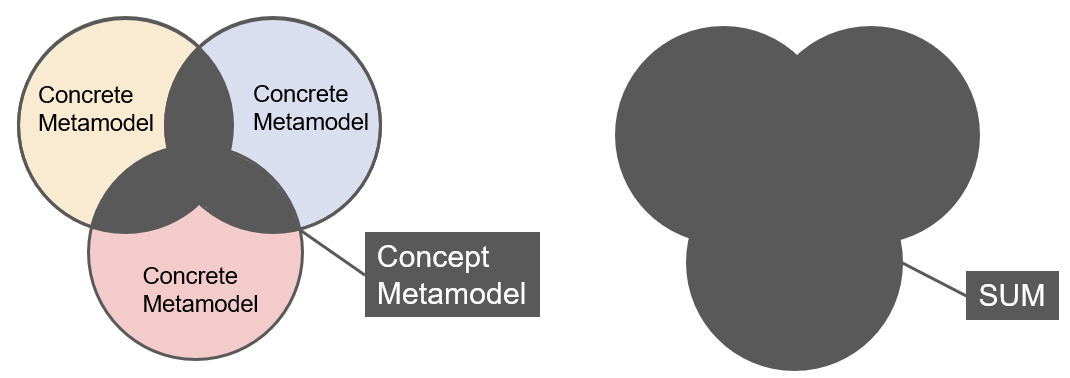
\includegraphics[width=\textwidth]{figures/quality/improvement/commonalities_and_sums.png}
    \caption[Commonalities compared to \acrlongpl{SUM}]{Sketched comparison for the scope of contents of \conceptmetamodels and \glspl{SUM}.}
    \label{fig:improvement:commonalities_and_sums}
\end{figure}

\mnote{Size of concept metamodels}
In general, a \conceptmetamodel has to contain \commonalities for all redundancies between the \concretemetamodels to keep consistent.
In a mathematical sense, this can be considered as the union of all pairwise intersections of the \concretemetamodels.
It can, however, not be precisely expressed as such, because elements may be similarly represented in the \concretemetamodels, but they are not the same.
One manifestation of the same \commonality may contain different information or encode it differently, such as using other units, than the others.
This already illustrates the essential difference to approaches in which one central model unifies all information about a system, called a \gls{SUM} (see \autoref{chap:foundations:multiview:osm}), from which the models used by different tools are derived by projections.
Such a \gls{SUM} can be seen as the union of all \concretemetamodels, whereas \concretemetamodels represent the union of their pairwise intersections, as illustrated in \autoref{fig:improvement:commonalities_and_sums}.


\subsection{Consistency Specification Types}
\label{chap:improvement:concepts:specification}

\mnote{Descriptive and normative specifications}
In \autoref{chap:networks:notions:normative_descriptive}, we have discussed the distinction of descriptive and normative specifications of consistency, which can be summarized as follows:
\begin{properdescription}
    \item[Descriptive Specification:] Descriptive specifications describe consistency relations that are \enquote{naturally} given when two metamodels represent common concepts redundantly or with common or dependent properties. 
    In that case, a notion of consistency already exists, formally or informally, to which the given specification must conform.
    This is, for example, the case for \gls{UML} class models and Java realizing object-oriented design.
    \item[Normative Specification:] Normative specifications prescribe consistency for metamodels for which no existing or common notion for consistency exists.
    This is especially the case if metamodels represent different abstractions or domains of a system, which have no implicit relations and for which different possibilities to relate them exist, such as an architecture description in \gls{PCM} and its implementation in Java.
\end{properdescription}
While descriptive consistency relations between two metamodels are usually definite, such as those for object-oriented design between \gls{UML} and Java, normative consistency relations may vary depending on the project context.
For example, several possible relations can be defined between an architecture description in \gls{PCM} and object-oriented design, such as the realization of each component as a class, as a bean in \glspl{EJB}, or as a complete project~\cite{langhammer2017a}.

\mnote{Suitability for descriptive specification}
Describing consistency by means of \commonalities and \conceptmetamodels especially promises to be useful for descriptive consistency specifications, where a \enquote{natural} relation exists due to elements representing common concepts.
It can, however, also be used to normatively define \commonalities in terms of a normative specification.
A component \commonality can, for example, define that a component manifests as a component in \gls{PCM} and as a class in \gls{UML} and Java, or, more generally, in an object-oriented design \conceptmetamodel.
This will, however, unlikely fit well for rather complex dependencies, such as a consistency relation requiring an implementation to fulfill some performance requirement.
In such a case, the complexity is in the specification of the relation anyway, which would have to be replicated when defining a \commonality between performance requirement and implementation.
Finally, this conforms to our distinction of structural and behavioral consistency relations given in \autoref{chap:networks:notions:types}, in which the \commonalities fit well for structural relations, on which we focus in this thesis anyway.

\mnote{Generalization}
In the following, we do not distinguish whether \commonalities are defined for common concepts that exist naturally, or for those which are prescribed by the definition of \conceptmetamodels and their \commonalities.
We will see that even for normative specifications \commonalities can be reasonably defined.
In \autoref{chap:improvement:application}, we also discuss how to combine ordinary transformations with the idea of \conceptmetamodels.


% \begin{copiedFrom}{VoSE}

% \section*{Running Example}

% We use a running example throughout the paper to explain the \commonalities idea.
% It relies on three metamodels: UML class models, Java code, whose grammar definition can be treated as a metamodel~\cite{heidenreich2010a}, and the \gls{PCM}~\cite{reussner2016a}, a component-based architecture description language.
% The consistency relations between Java and UML class models are mostly one-to-one mappings, as they provide the same concepts of object-oriented design. %provide redundant representations of the same concepts, so the consistency relations between them define mostly one-to-one mappings.
% Consistency relations between \gls{PCM} and Java were proposed by \textcite{langhammer2015a}.
% For this paper, only the one-to-one mapping between components in \gls{PCM} and classes in Java---or generally all object-oriented languages---are relevant, whereby each component is mapped to a class but not vice versa.

% For the examples in this paper, a minimalist subset of those metamodels, depicted in \autoref{fig:improvement:running_example}, is sufficient.
% It only comprises classes in UML and Java and components in \gls{PCM}, which all have a name.
% The name shall be equal between corresponding classes in UML and Java, whereas the classes realizing a component shall have the same name as the component, complemented by an \enquote{Impl} suffix (see~\cite{langhammer2015a}).
% With state-of-the-art techniques, those constraints could be implemented as relations in declarative or as enforcing routines in imperative transformation languages.

% \begin{figure}
% 	\centering
% 	\newcommand{\vdistance}{7.5em}
\newcommand{\hdistance}{(18em+0.4*\difftoafiveimage)}
\newcommand{\classwidth}{5.5em}
\newcommand{\labeldistance}{0.2em}
\newcommand{\mmborder}{1.5em}


\begin{tikzpicture}

\pgfdeclarelayer{bg}
\pgfsetlayers{bg,main}


% METACLASSES

\umlclassvarwidth{java_class}{}{Class}{
name\\
}{\classwidth}  

\umlclassvarwidth[, below=\vdistance of java_class.center, anchor=center]{uml_class}{}{Class}{
name\\
}{\classwidth} 

\umlclassvarwidth[, below left=0.5*\vdistance and \hdistance of java_class.center, anchor=center]{pcm_component}{}{Component}{
name\\
}{\classwidth} 


% METAMODELS

\coordinate (java_label_coordinate) at ([yshift=\labeldistance]java_class.north);
\node[mmlabel, anchor=south] (java_label) at (java_label_coordinate) {Java};

\coordinate (uml_label_coordinate) at ([yshift=-\labeldistance]uml_class.south);
\node[mmlabel, anchor=north] (java_label) at (uml_label_coordinate) {\acrshort{UML}};

\coordinate (pcm_label_coordinate) at ([xshift=-7*\labeldistance]pcm_component.west);
\node[mmlabel, right=6*\labeldistance of pcm_label_coordinate, anchor=east] (pcm_label) {\acrshort{PCM}};

\begin{pgfonlayer}{bg}
    \node[mmbg, fit=(java_class)(java_label_coordinate), inner sep=\mmborder] (java) {};
    \node[mmbg, fit=(uml_class)(uml_label_coordinate), inner sep=\mmborder] (uml) {};
    \node[mmbg, fit=(pcm_component)(pcm_label_coordinate), inner sep=\mmborder] (pcm) {};
\end{pgfonlayer}


% CONSISTENCY RELATIONS

\draw[directed consistency relation] (pcm_component) |- node[pos=0, above left] {$\mathvariable{co}$} node[above, pos=0.65, align=center] {$\setted{\tupled{\mathvariable{co}, \mathvariable{cl}} \mid \mathvariable{cl.name} = \mathvariable{co.name} + "\mathvariable{Impl}"}$} node[pos=1, below left] {$\mathvariable{cl}$} (java_class);
\draw[consistency relation] (java_class) -- node[pos=0, below right] {$\mathvariable{jcl}$} node[left] {$\setted{\tupled{\mathvariable{jcl}, \mathvariable{ucl}} \mid \mathvariable{jcl.name} = \mathvariable{ucl.name}}$} node[pos=1, above right] {$\mathvariable{ucl}$} (uml_class);
\draw[directed consistency relation] (pcm_component) |- node[pos=0, below left] {$\mathvariable{co}$} node[below, pos=0.65, align=center] {$\setted{\tupled{\mathvariable{co}, \mathvariable{cl}} \mid \mathvariable{cl.name} = \mathvariable{co.name} + "\mathvariable{Impl}"}$} node[pos=1, above left] {$\mathvariable{cl}$} (uml_class);

\end{tikzpicture}

% 	\caption[Consistency relations for extracts of Java, UML and PCM]{Simple metamodel extracts for Java, UML and \gls{PCM} and consistency relations between them.}
% 	\label{fig:improvement:running_example}
% \end{figure}

% In this paper, we consider metamodels that conform to the \gls{EMOF} standard~\cite{mof}.
% Such metamodels consist of classes, which we denote as \emph{\metaclasses} to avoid confusion with classes in exemplary metamodels such as Java and UML.
% \Metaclasses can in turn contain attributes and associations to other classes, which may be containments.


% \subsection*{Making Common Concepts Explicit}

% The redundancies between different metamodels are an expression of common concepts that are represented redundantly.
% We already gave the example of a class in UML and Java, which are different representations of the common concept of a class in general object-oriented design.
% We propose to make common concepts explicit rather than encoding them into the rules of a transformation.
% This can be achieved by creating a \emph{\conceptmetamodel}, which defines those common concepts, and specifying the relations between the \conceptmetamodel and the existing metamodels.
% We refer to the existing metamodels as \emph{\concretemetamodels}.
% The relation specifications can be used to derive transformations between the \concretemetamodels and the \conceptmetamodel.

% \autoref{fig:quality:commonalities_example} shows the \metaclasses for a \texttt{Class} as extracts of the \concretemetamodels for UML and Java and the \metaclass for the common concept of a \texttt{Class} in the \conceptmetamodel for object-oriented design.
% We denote a single common concept as a \emph{\commonality}.
% Further \commonalities in object-oriented design could, for example, be interfaces or methods.
% The relation between the \texttt{Class} \commonality and its realizations in the \concretemetamodels are shown by a \emph{«manifests»} relation.
% %Such a relation can be defined in a transformation.
% In our simplified example, the relation would especially define that the names of the classes have to be equal. %an equality relationship.

% \begin{figure}
%     \centering
%     \newcommand{\vdistance}{7.5em}
\newcommand{\hdistance}{11em}
\newcommand{\classwidth}{5.5em}
\newcommand{\labeldistance}{1.2em}
\newcommand{\labelshift}{0.3*\classwidth}
\newcommand{\representstext}{\emph{«manifests»}}
\newcommand{\mmborder}{1em}

\begin{tikzpicture}

\pgfdeclarelayer{bg}
\pgfsetlayers{bg,main}


% METACLASSES

\umlclassvarwidth{java_class}{}{Class}{
name\\
}{\classwidth}  

\umlclassvarwidth[, right=\hdistance of java_class.north, anchor=north]{uml_class}{}{Class}{
name\\
}{\classwidth} 

\umlclassvarwidth[, above right=\vdistance and 0.5*\hdistance of java_class.north, anchor=north]{oo_class}{}{Class\vphantom{p}}{
name\\
}{\classwidth} 


% METAMODELS

\coordinate (java_label_coordinate) at ([xshift=-\labelshift,yshift=\labeldistance]java_class.north);
\node[mmlabel, anchor=center] (java_label) at (java_label_coordinate) {Java};

\coordinate (uml_label_coordinate) at ([xshift=\labelshift,yshift=\labeldistance]uml_class.north);
\node[mmlabel, anchor=center] (java_label) at (uml_label_coordinate) {UML};

\coordinate (oo_label_coordinate) at ([yshift=\labeldistance]oo_class.north);
\node[mmlabel, anchor=center] (oo_label) at (oo_label_coordinate) {Object-oriented Design};

\begin{pgfonlayer}{bg}
    \node[mmbg, fit=(java_class)(java_label_coordinate), inner sep=\mmborder] (java) {};
    \node[mmbg, fit=(uml_class)(uml_label_coordinate), inner sep=\mmborder] (uml) {};
    \node[conceptmmbg, minimum width=11.5em, fit=(oo_class)(oo_label_coordinate), inner sep=\mmborder] (oo) {};
\end{pgfonlayer}


% CONSISTENCY RELATIONS

\draw[consistencyrel, <-] (java_class) -- node[above, sloped] {\representstext} (oo_class);
\draw[consistencyrel, <-] (uml_class) -- node[above, sloped] {\representstext} (oo_class);

\end{tikzpicture}

%     \caption[Concept metamodel for object-oriented design]{\Conceptmetamodel for object-oriented design with a \texttt{Class} \commonality and its relations to UML and Java.}
%     \label{fig:quality:commonalities_example}
% \end{figure}

% When another \concretemetamodel that represents the same concepts shall be added, it is only necessary to define its relation to the \conceptmetamodel.
% For example, adding \cplusplus as another metamodel representing object-oriented design would require the definition of the relation between the \texttt{Class} \commonality in object-oriented design and its representation in \cplusplus.
% Adding an additional metamodel may require the \conceptmetamodel to be extended by \commonalities that were not relevant for the already considered metamodels.
% In general, a \conceptmetamodel has to contain \commonalities for redundancies in all \concretemetamodels, which---mathematically speaking---can be expressed as the union of all pairwise intersections of the \concretemetamodels.

% Short description of the Commonalities concept and application to example (UML and Java classes, could e.g., be extended by C++)
% Necessary artifacts: the Commonalities metamodel and the transformations.
% But: one can define a language to specify the Commonalities metamodel together with a specification of how the elements and properties manifest in the concrete metamodels, which we will explain in more detail in \autoref{sec:language}.
% Introduce terms: \emph{Commonality} (metamodel with common concepts), concrete metamodel (a metamodel that is accessed by a user) and \emph{Manifestation} (the concrete metamodels that realize a Commonality).
% \end{copiedFrom} % VoSE


% \begin{copiedFrom}{DocSym}

% \section*{Making Common Concepts Explicit} 

% \subsection{Approach
%     \pgsize{1 p.}
%     \dl{16.06.2017}
%     \complete{0}}

%\todoConference{A description of the proposed solution and which other work (e.g., methods or tools) it depends on.}
%\todoHeiko{One Solution: Add additional models. Already proposed by Stevens, but just to solve constraints. Here, we make overlaps explicit}
%\todo{Referenz zu Aussage von Stevens hinzufügen}
%\todoHeiko{Discuss necessity to provide orthogonal concept metamodels}

%\todoHeiko{Why ''virtual``? Because they are transparent to the user and nothing he has to deal with}
%\todo{Referenz auf Grafik und Optimalfall davon erklären}
% Based on the decomposition of consistency relations, we propose another approach to achieve a tree structure of transformations, which inherently optimizes \emph{modularity}.
%In the following, we propose another solution option to achieve a tree structure of consistency relations, next to decomposing consistency relations into independent subsets.
%This approach called \emph{\acp{CMM}} ensures consistency between specifications inherently given by the tree structure, but also optimizes modularity, so that an arbitrary subset of the metamodels can be used.
%It also reuses the concepts for decomposing consistency relations.
% In \autoref{sec:Introduction}, we discussed reasons for specifying consistency using binary transformations instead of defining multiary relations.
% Nevertheless, as discussed in the previous section, trade-off decisions regarding the identified challenges have to made with that approach.
% Therefore, we propose an approach called \emph{\acp{CMM}} for a certain kind of relations that addresses all those identified challenges.
% The idea bases on the insight that we can distinguish two kinds of consistency relations:
% \begin{description}[leftmargin=\parindent]
%     \item[Descriptive consistency relations] are \enquote{naturally} given when two metamodels represent common \emph{concepts} %with common properties
%     redundantly or at least with dependent properties. This is, for example, the case for \gls{UML} class models and Java realizing \gls{OO}. %, and for \ac{UML} component models and \ac{PCM} models realizing a component concept.
%     %They have to be expressed by transformations in a way that they describe the underlying consistency relations.
%     \item[Normative consistency relations] prescribe consistency and %are induced by transformations and that 
%     do not exist \enquote{naturally}. This is especially the case if metamodels represent different abstractions or domains of a system, which have no implicit relation, such as an \gls{ADL} and Java. % in our example.
% \end{description}

% While descriptive consistency relations between two metamodels are usually definite, such as those between \gls{OO} design in \gls{UML} and Java, normative consistency relations may vary depending on the project context.
% For example, several possible relations can be defined between an \gls{ADL} and \gls{OO} design, for example the realization of each component as a class or as a complete project~\cite{langhammer2017a}.
%$For example, the relation between \ac{OO} design in \ac{UML} and Java will usually be definite and not depend on the context, whereas there may be several possible relations between an \ac{ADL} and OO-design.
%Depending on the context, a component could be realized by a class or a complete project, and a class realizing an architectural component may be placed anywhere or in a specific package, as discussed by \textcite{langhammer2017a}.

% Transformations for descriptive consistency relations implicitly encode %the preservation of consistency between 
% the common concepts.
% %Descriptive consistency relations base on the fact that different metamodels represent similar or equal concepts.
% %In consequence, transformations are supposed to define the preservation of consistency between those common concepts.
% %Instead of implicitly encoding those common concepts in transformations, 
% Instead, we propose to make these common concepts explicit in so-called \emph{\glspl{CMM}} and define relations between them and the concrete metamodels.
% We illustrate this in \autoref{fig:quality:concept_metamodel_integration}.
% The descriptive consistency relation \ref{fig:quality:concept_metamodel_integration:R1} is converted into a \gls{CMM} for the metamodels \ref{fig:quality:concept_metamodel_integration:A} and \ref{fig:quality:concept_metamodel_integration:B} with new relations \ref{fig:quality:concept_metamodel_integration:R4} and \ref{fig:quality:concept_metamodel_integration:R5} between the concrete metamodels and the \gls{CMM}.
% The existing normative consistency relations \ref{fig:quality:concept_metamodel_integration} and \ref{fig:quality:concept_metamodel_integration:R3} to metamodel \ref{fig:quality:concept_metamodel_integration:C} are replaced by a new relation \ref{fig:quality:concept_metamodel_integration:R6} to the \gls{CMM}. % to the metamodel \ref{fig:concept:C}.
% The \gls{CMM} and its consistency relations have to be appropriately defined to replace the original ones, as depicted in \autoref{fig:quality:concept_metamodel_integration}. %, have to be fulfilled by appropriately defining the \ac{CMM}.
% It will be part of our research to figure out how to define such a \gls{CMM}, so that it can also be combined with other metamodels. %, without estimating the additional information that may be necessary in the \ac{CMM} a-priori.
% While it basically has to contain the common concepts of the metamodels sharing a descriptive consistency relations, it may also need to contain additional information depending on consistency relations to other metamodels, which are not known a-priori.

% \begin{figure}
%     \centering
%     \newcommand{\mmdistance}{8em}

\begin{tikzpicture}[
    mm/.style={draw, circle, fill=lightgray, inner sep=0.25em},
    consistencyrel/.style={latex-latex,dashed}]


\node[mm] (original_left) {\mylabel{fig:quality:concept_metamodel_integration:A}{$A$}};
\node[mm, right=\mmdistance of original_left.center, anchor=center] (original_middle) {\mylabel{fig:quality:concept_metamodel_integration:B}{$B$}};
\node[mm, right=\mmdistance of original_middle.center, anchor=center] (original_right) {\mylabel{fig:quality:concept_metamodel_integration:C}{$C$}};

\draw[consistencyrel] (original_left) -- node[above] {\mylabel{fig:quality:concept_metamodel_integration:R1}{$R_1$}} node[below] {\textit{descriptive}} (original_middle);
\draw[consistencyrel] (original_middle) to[bend left=30] node[above] {\mylabel{fig:quality:concept_metamodel_integration:R2}{$R_2$}} node[below=0.2em] {\textit{normative}} (original_right);
\draw[consistencyrel] (original_left) to[bend right=40] node[above] {\mylabel{fig:quality:concept_metamodel_integration:R3}{$R_3$}} node[below] {\textit{normative}} (original_right);


\node[mm, fill=gray!10, above right=0.55*\mmdistance and 0.5*\mmdistance of original_left.center, anchor=center, align=center] (concept) {$AB-$\\$CMM$};

\draw[consistencyrel, color=gray] (original_left) -- node[above left=-0.3em and 0.5em] {\mylabel{fig:quality:concept_metamodel_integration:R4}{$R_4$}} (concept);
\draw[consistencyrel, color=gray] (original_middle) -- node[above right=-0.3em and 0.3em] {\mylabel{fig:quality:concept_metamodel_integration:R5}{$R_5$}} (concept);
\draw[consistencyrel, color=gray] (original_right) to[bend right=30] node[pos=0.6, below left] {\mylabel{fig:quality:concept_metamodel_integration:R6}{$R_6$}} (concept);



\node[right=2.5*\mmdistance of concept.north, anchor=north east, align=left] { 
$R_1 \concat R_2 \neq (R_1 \concat R_2) \cap R_3 \neq R_3$
};

\node[below right=2em and 2.5*\mmdistance of concept.north, anchor=north east, align=left] {
$R_4 \concat R_5 = R_1$\\
$R_4 \concat R_6 = R_3$\\
$R_5 \concat R_6 = R_2$\\
};


\end{tikzpicture}
%     \caption{Definition of a concept metamodel}
%     \label{fig:quality:concept_metamodel_integration}
%     \todo{We can use this for showing how to integrate commonalities with ordinary direct relations, maybe there should be a section about that.}
% \end{figure}

%%%As one concrete example, instead of specifying transformations between \ac{OO} design in \ac{UML} and Java, an OO-\ac{CMM}, with concepts like classes, inheritance and so on, and the relations of \ac{UML} and Java to this \ac{CMM} could be defined.
% These concept metamodels can be seen as additional metamodels 
% of metamodels having inherent consistency relations explicit within a \ac{VOMM} and to define a mapping between concrete metamodels and \acp{VOMM}. We claim that prescribed consistency is actually not specific for concrete metamodels, but for concepts as represented by our \acp{VOMM}, which means that metamodels with prescribed consistency relations can be kept consistent by specifying consistency preservation between their \acp{VOMM}. In our example, this means that consistency relations between \ac{PCM} and Java should be expressed as relations between OO and component concept. 

%%%%% CBSE-EXAMPLE REMOVED!
% In \autoref{fig:cmm_example}, we illustrate the usage of such \acp{CMM} to define an OO-concept and a concept for component-based architecture descriptions, relating component models of \ac{UML} and the \acf{PCM} to.
% Relations between those \acp{CMM} can again be defined using other \acp{CMM}, or by defining ordinary transformations between them. 
% We discuss the impact of that decision in the following.

% \begin{figure}
%     \vspace{-0.7em}
%     \begin{center}
%         \input{figures/cmm_example.tex}
%     \end{center}
%     \vspace{-0.7em}
%     \caption{Exemplary \acp{CMM} and their consistency relations}
%     \label{fig:cmm_example}
% \end{figure}

%\todoHeiko{Das mit der Baumstruktur ist ein Knackpunkt. Kommt der gut genug rüber?}
% To avoid the drawbacks of transitive transformation execution between \acp{VOMM}, it is necessary that only one propagation path between two metamodels exists. This requires to define \ac{VOMM} relations in a way such that they induce an an acyclic graph by also extracting common concepts of \acp{VOMM} in another \ac{VOMM}. 
%In the example, the component \ac{VOMM} could be seen as an abstracted concept of the OO \ac{VOMM}. 
% It will be part of our research to identify if such an ordering of concepts can be achieved in different case studies.

%%% REMOVED THE FOLLOWING, AS NOT A RELEVANT "DRAWBACK"
%Such \acp{CMM} are technically similar to introducing new metamodels and defining transformations between them and existing metamodels.
%Nevertheless, they are conceptually different.
%First, they are supposed to be transparent to the user of the concrete models.
%Additionally, 
% This approach addresses all identified challenges % identified in \autoref{sec:approach:challenges} 
% and solves them under the assumption that all consistency relations %of a system 
% are described using \glspl{CMM}. %if their specification is encapsulated in a specialized language, our challenges identified in \autoref{sec:approach:challenges} can be addressed.
% %Under the assumption that all consistency relations of a system can be described using \acp{CMM}, we would be able to solve all identified challenges, as using \acp{CMM} allows to have the expressiveness of a graph of transformations, but abstracted to a tree structure with all its advantages.
% %We achieve \emph{uniqueness} by extracting common concepts into \acp{CMM} having to define only one relation of a metamodel to the \ac{CMM}. 
% We achieve inherent transformation compatibility by avoiding more than one transformation path %for the propagation of one change 
% between two metamodels by design. %Therefore, it is necessary to define \acp{CMM} relations in a way such that they induce a tree by also extracting common concepts of \acp{CMM} in other \acp{CMM}.  
% Since metamodels are only coupled across \glspl{CMM} and thus represent leaves of the transformation tree, any subset of them can be selected, maximizing modularity. % can be performed in a concrete usage scenario, maximizing modularity.
% %Finally, we assume that expressing consistency with explicit common concepts improves comprehensibility, %over combining binary consistency specifications
% %as it is a more natural representation and especially no transformations paths have to be traversed to understand a specific relation. % and expressing common information in common concepts is more natural than expressing it in transformations.
% %An approach of adding additional metamodels is also shortly discussed in \cite{stevens2020BidirectionalTransformationLarge-SoSym}, but with the focus on definability of multiary relations rather than the optimization regarding certain challenges.
% Finally, we assume that making common concepts explicit improves comprehensibility.

% The most crucial part of this approach is the necessity to build a tree of \glspl{CMM}.
% This will not be possible if always considering whole metamodels and their relations, but can be possible if independent concepts are extracted to be treated individually.
% For that, we will apply our findings on consistency relation decomposition (see \autoref{chap:commonalities:approach}).
% %This is similar to decomposing consistency relations, as introduced in \autoref{sec:approach:decomposition}, which is why we will apply our findings therefrom.
% Additionally, the approach specifically aims to improve the specification of transformations for descriptive relations.
% In consequence, it must be combined with transformations expressing the normative relations between \glspl{CMM} and other metamodels.

% Introduction of the \emph{MultiCons} approach for consistency between multiple, heterogeneous models with the specification of virtual overlap metamodels.

% \begin{itemize}
%     \item Why do we keep two models consistent?
%     \begin{enumerate}
%         \item They represent a common \emph{concept} with common properties of the system under development, which induces their redundant representation or at least dependencies between properties of the models, e.g., both UML class models and Java code realize an OO-concept.
%         \item They represent different abstractions of or views on a system, but a prescription of consistency preservation rules exists. For example, for descriptions of the component-based software architecture with the Palladio Component Model (PCM) and Java code a consistency specification was developed by \textcite{langhammer2017a}.
%     \end{enumerate}
%     \item We call this overlap of information that is represented in several models and that requires consistency preservation a \emph{semantic overlap}, as models overlap because they contain information with the same or dependent semantics.
%     \item Currently, consistency preservation tools require the specification of relations between two models, which implicitly defines the common properties. E.g., specifying the relations between Java code and UML class models implicitly contains a specification of the common properties of both metamodels
%     \item Idea: 
%     \begin{enumerate}
%         \item Make the common properties explicit in \emph{virtual overlap metamodels (VOMMs)} and define how these properties map to the concrete properties of existing metamodels
%         \item Define consistency relations between metamodels representing different abstractions or views on the systems between VOMMs rather than the actual metamodels.
%     \end{enumerate}
% \end{itemize}



% Envisioned benefits of this approach are:
% \begin{itemize}
%     \item Reduction of risk of inconsistent consistency specifications by design and thus reductions of risk of propagation cycles: Refer to challenge in introduction
%     \item Modular consistency specifications: Relations between two metamodels are defined across VOMMs, such that single metamodels can be omitted without losing necessary consistency relations (transitive relations)
%     \item Comprehensibility: Defining common concepts and their relations is (hopefully) better comprehensible than defining relations between pairs of metamodels
% \end{itemize}

% Known drawbacks:
% \begin{itemize}
%     \item Specification is more elaborate in simple cases (two metamodels only), as the VOMM has to be defined additionally
%     \item 
% \end{itemize}

% \end{copiedFrom} % DocSym

\section{The \commonalities Approach}
\label{chap:improvement:commonalities}

\mnote{Approach overview}
We have motivated the idea of representing common concepts of redundantly or dependently represented elements of different metamodels in terms of \commonalities in explicit \conceptmetamodels rather than implicitly encoding them in direct consistency relations between the metamodels.
In the following, we discuss the specification of \conceptmetamodels and the notion of manifestation relations in more detail.
We also depict how further benefits can be generated by composing \conceptmetamodels in terms of defining a hierarchy of them.
We call this approach of defining and composing \conceptmetamodels of \commonalities the \emph{\commonalities approach}.
Essential for the central benefit of this approach, which is mitigation of trade-offs between quality properties of transformation networks, is the inherent possibility to achieve a specific kind of tree topology, which we derive from the approach before discussing different options for its operationalization.


\subsection{Concept Metamodels}

\mnote{Structure of metamodels}
The inherent benefits of the \commonalities approach are given by the definition of additional \conceptmetamodels, across which consistency relations are expressed, instead of defining consistency relations between the \concretemetamodels.
How these \conceptmetamodels and the manifestation relations between them and the \concretemetamodels look like is not that relevant.
Still, we discuss how elements can represented as \commonalities in a \conceptmetamodel and which situations instead of pure redundancies representing exactly the same information as in the manifestation can exist.

\begin{figure}
    \centering
    \newcommand{\vdistance}{12em}
\newcommand{\hdistance}{23em}
\newcommand{\innerhdistance}{7.6em}
\newcommand{\classwidth}{4.7em}
\newcommand{\labeldistance}{0.9em}
\newcommand{\mmborder}{0.9em}
\newcommand{\referenceshift}{0.9em}

\begin{tikzpicture}

\pgfdeclarelayer{bg}
\pgfsetlayers{bg,main}


% METACLASSES

\umlclassvarwidth{java_class}{}{Class}{
name\\
packageName
}{\classwidth}  

\umlclassvarwidth[, right=\innerhdistance of java_class.north, anchor=north]{java_field}{}{Field}{
name\\
}{\classwidth} 

\umlassociationfromto{([yshift=\referenceshift]java_field.west-|java_class.east) -- node[uml cardinality start, pos=0, above right] {$1$} node[uml cardinality end, pos=1, above left] {$*$} ([yshift=\referenceshift]java_field.west)}
\umlassociationfromto{([yshift=-\referenceshift]java_field.west) -- node[uml cardinality start, pos=0, above left] {$*$} node[uml role end, pos=1, below right] {type} node[uml cardinality end, pos=1, above right] {$1$} ([yshift=-\referenceshift]java_field.west-|java_class.east)}

\umlclassvarwidth[, below right=5em and \hdistance of java_class.north, anchor=north]{uml_class}{}{Class}{
name\\
}{\classwidth} 

\umlclassvarwidth[, left=\innerhdistance of uml_class.north, anchor=north]{uml_association}{}{Association}{
name\\
}{\classwidth}

\umlclassvarwidth[, above=5em of uml_class.north, anchor=north]{uml_package}{}{Package}{
name\\
}{\classwidth}

\umlassociationfromto{([yshift=\referenceshift]uml_association.east) -- node[uml cardinality start, pos=0, above right] {$*$} node[uml role end, pos=1, below left] {from} node[uml cardinality end, pos=1, above left] {$1$} ([yshift=\referenceshift]uml_class.west)}
\umlassociationfromto{([yshift=-\referenceshift]uml_association.east) -- node[uml cardinality start, pos=0, above right] {$*$} node[uml role end, pos=1, below left] {to} node[uml cardinality end, pos=1, above left] {$1$} ([yshift=-\referenceshift]uml_class.west)}
\umlassociationfromto{(uml_package.south) -- node[uml cardinality start, pos=0, below left] {$1$} node[uml role end, pos=1, above right] {classes} node[uml cardinality end, pos=1, above left] {$*$} (uml_class.north)}

\umlclassvarwidth[, above right=\vdistance and 0.5*\hdistance-0.5*\innerhdistance of java_class.north, anchor=north]{oo_class}{}{Class\vphantom{p}}{
name\\
}{\classwidth} 

\umlclassvarwidth[, below=5em of oo_class.north, anchor=north]{oo_association}{}{Association}{
name\\
}{\classwidth}

\umlclassvarwidth[, right=1.2*\innerhdistance of oo_class.north, anchor=north]{oo_package}{}{Package}{
name\\
}{\classwidth}

\umlassociationfromto{([xshift=-0.8*\referenceshift]oo_class.south) -- node[uml cardinality start, pos=0, below right] {$1$} node[uml role end, pos=0, below left] {from} node[uml cardinality end, pos=0, above right] {$*$} ([xshift=-0.8*\referenceshift]oo_association.north)}
\umlassociationfromto{([xshift=1.2*\referenceshift]oo_association.north) -- node[uml cardinality start, pos=0, above left] {$*$} node[uml role end, pos=1, below right] {to} node[uml cardinality end, pos=1, below left] {$1$} ([xshift=1.2*\referenceshift]oo_class.south)}
\umlassociationfromto{(oo_package.west) -- node[uml cardinality start, pos=0, below left] {$1$} node[uml role end, pos=1, above right] {classes} node[uml cardinality end, pos=1, below right] {$*$} (oo_class.east)}


% METAMODELS

\coordinate (java_label_coordinate) at ([yshift=\labeldistance]java_class.north west);
\node[mmlabel, anchor=west] (java_label) at (java_label_coordinate) {Java};

\coordinate (uml_label_coordinate) at ([yshift=\labeldistance]uml_package.north east);
\node[mmlabel, anchor=east] (java_label) at (uml_label_coordinate) {UML};

\coordinate (oo_label_coordinate) at ([yshift=\labeldistance]$(oo_class.north)!0.5!(oo_package.north)$);
\node[mmlabel, anchor=center] (oo_label) at (oo_label_coordinate) {Object-oriented Design};

\begin{pgfonlayer}{bg}
    \node[mmbg, fit=(java_class)(java_field)(java_label_coordinate), inner sep=\mmborder] (java) {};
    \node[mmbg, fit=(uml_class)(uml_package)(uml_association)(uml_label_coordinate), inner sep=\mmborder] (uml) {};
    \node[conceptmmbg, minimum width=11.5em, fit=(oo_class)(oo_association)(oo_package)(oo_label_coordinate), inner sep=\mmborder] (oo) {};
\end{pgfonlayer}


% CONSISTENCY RELATIONS

\draw[manifests relation] ([xshift=-0.48*\classwidth]oo_class.south) -- node[manifests relation, above, sloped] {\manifestslabel} (java_class);
\draw[manifests relation] ([xshift=0.48*\classwidth]oo_class.south) -- node[manifests relation, above, sloped] {\manifestslabel} (uml_class);
\draw[manifests relation] (oo_association) -- node[manifests relation, above, sloped] {\manifestslabel} (java_field);
\draw[manifests relation] (oo_association) -- node[manifests relation, above, sloped] {\manifestslabel} (uml_association);
\draw[manifests relation] (oo_package) -- node[manifests relation, above, sloped] {\manifestslabel} (uml_package);

\end{tikzpicture}

    \caption[Multiple \commonality example for object-oriented design]{\Conceptmetamodel for object-oriented design with a \texttt{Class}, an \texttt{Association} and a \texttt{Package} \commonality and its relations to the \concretemetamodels \gls{UML} and Java with a different representation of associations as fields and packages as attributes of classes in Java.}
    \label{fig:improvement:multiple_commonalities_example}
\end{figure}

\mnote{Representation of packages}
\autoref{fig:improvement:multiple_commonalities_example} depicts an extension of the example given in \autoref{fig:improvement:one_commonality_example}.
In addition to classes, it contains the representation of packages and associations.
A package is represented as a dedicated \metaclass in \gls{UML}, which references the classes contained in that package.
Java, however, does not have an explicit representation of packages, but encodes them into the package names specified within classes and, additionally, represents them in a folder structure in which the source code files of the classes are persisted.
A \conceptmetamodel used to preserve consistency between packages represented in \gls{UML} and Java must represent this information in any way such that changes in Java code can be propagated into a \gls{UML} model to preserve their consistency and vice versa.
To sketch an extreme, this could even be achieved with some string attribute in the \conceptmetamodel that encodes this information in such a unique way that the necessary information for both instances of the \concretemetamodels can be generated.
Actually, a \conceptmetamodel should represent such information in a reasonable structure, whose concrete characteristics have to be defined the transformation developer.
For packages, either the representation in Java as attributes of classes or the representation in \gls{UML} as a dedicated \metaclass can be chosen.
In the given example, we define packages in the \conceptmetamodel as explicit \metaclasses, as this makes the containment structure of classes in packages explicit.
In addition, in the complete \gls{UML} and Java metamodel packages are represented hierarchically, which is also easier to express as a relation between dedicated elements rather than their implicit encoding in the package names of classes.

\mnote{Representation of associations}
Associations in \gls{UML} are used to define that classes are related to each other.
Each association defines two classes, denoting from which class to which class the association is defined.
Java does not provide an explicit representation of associations, which usually results in their implicit representation as fields of the class from which the association is defined and having the type of the class to which it is defined.
In the example, we have chosen to represent an association explicitly in the \conceptmetamodel.
Fields can, in the complete Java and \gls{UML} metamodels, be related to further elements than associations, thus having this distinction within the \conceptmetamodel gives it more semantics.
In addition, we have chosen to have the class from which the association is defined reference the association instead having this reference in the opposite direction as in the \gls{UML} metamodel.
No matter whether or not this is beneficial, still all necessary information to keep Java fields and \gls{UML} associations consistent is represented by the \conceptmetamodel.
It shows that for the \conceptmetamodel even a representation that differs from all its manifestations can be chosen.

\mnote{General rule for \conceptmetamodels}
As mentioned before, the only requirement to a \conceptmetamodel is that it must be able to represent all information that is necessary for defining manifestation relations to the \concretemetamodels, such that they are able to preserve consistency according to some consistency relation between the \concretemetamodels.
A general, but rather informal rule, which has proven to be beneficial in the implementation of a case study for our evaluation, is to select among different representation options the semantically richest.
In the example, we have thus chosen to represent packages explicitly instead of implicitly encoding them in package names of classes.
This improves expressiveness of the \conceptmetamodel and makes its information easier to use for defining manifestation relations without interpreting implicitly encoded information in each of these relations.


\subsection{Composition of Concepts}

\mnote{Multiple \commonalities}
We have so far discussed the idea of defining an additional \conceptmetamodel to represent the common concepts of two or more \concretemetamodels.
For the depicted example for Java and \gls{UML}, it seems reasonable to define the group the common concepts in object-oriented design in such a metamodel.
In \autoref{fig:improvement:running_example}, we have also considered \gls{PCM} components and their consistency relations to classes in \gls{UML} and Java.
Although we could define a component \commonality for \gls{PCM} components and classes in \gls{UML} and Java, and consider this \commonality next to the class \commonality for classes in \gls{UML} and Java, we will likely not do so because of several drawbacks.
First, a component \commonality does, semantically, not fit into the discussed \conceptmetamodel for object-oriented design. Thus, the \conceptmetamodel would have to be considered broader, potentially only as a generic \conceptmetamodel.
Second, and more importantly, such a construction would introduce further redundancies, as the relation between classes in \gls{UML}and Java is expressed via two \commonalities, once the class \commonality and once the component \commonality.

\mnote{Monolithic \commonalities}
To solve the problem of a redundant specification of the relation between classes in \gls{UML} and Java via class and component \commonalities, we could combine these two \commonalities to a single one, representing all necessary common information.
If, however, further elements share information with classes and components, they also have to be merged into the same \commonality.
In the extreme case, this could result in only having one large \commonality that is able to represent all related information.
The manifestation relations would then have to make all kinds of distinctions based on the information given in such a \commonality.

\mnote{Exemplary \commonality hierarchy}
An intuitive solution for the example scenario is to not consider classes in \gls{UML} and Java as manifestations of a component \commonality, but to consider the class \commonality as a manifestation of the component \commonality.
Then the relation between classes in \gls{UML} and Java is still represented across one specific class \commonality, whereas the manifestation relation of the component \commonality only has to be defined for the concept of classes instead of their concrete manifestations.

\begin{figure}
    \centering
    \newcommand{\vdistance}{7em}
\newcommand{\hdistance}{13em}
\newcommand{\classwidth}{5.5em}
\newcommand{\labeldistance}{1em}
\newcommand{\labelshift}{0.3*\classwidth}
\newcommand{\mmborder}{1em}

\begin{tikzpicture}

\pgfdeclarelayer{bg}
\pgfsetlayers{bg,main}


% METACLASSES

\umlclassvarwidth{java_class}{}{Class}{
name\\
}{\classwidth}  

\umlclassvarwidth[, right=0.8*\hdistance of java_class.north, anchor=north]{uml_class}{}{Class}{
name\\
}{\classwidth} 

\umlclassvarwidth[, above right=\vdistance and 0.5*\hdistance of java_class.north, anchor=north]{oo_class}{}{Class\vphantom{p}}{
name\\
}{\classwidth} 

\umlclassvarwidth[, right=\hdistance of oo_class.north, anchor=north]{pcm_component}{}{Component}{
name\\
}{\classwidth} 

\umlclassvarwidth[, above right=\vdistance and 0.5*\hdistance of oo_class.north, anchor=north]{component_component}{}{Component}{
name\\
}{\classwidth}

% METAMODELS

\coordinate (java_label_coordinate) at ([yshift=\labeldistance]java_class.north west);
\node[mmlabel, anchor=west] (java_label) at (java_label_coordinate) {Java};

\coordinate (uml_label_coordinate) at ([yshift=\labeldistance]uml_class.north east);
\node[mmlabel, anchor=east] (uml_label) at (uml_label_coordinate) {\acrshort{UML}};

\coordinate (oo_label_coordinate) at ([xshift=-4*\labelshift,yshift=\labeldistance]oo_class.north);
\node[mmlabel, anchor=west, align=left] (oo_label) at ([xshift=-0.5em, yshift=-0.7em]oo_label_coordinate) {Object-oriented\\ Design};

\coordinate (pcm_label_coordinate) at ([yshift=\labeldistance]pcm_component.north east);
\node[mmlabel, anchor=east] (pcm_label) at (pcm_label_coordinate) {\acrshort{PCM}};

\coordinate (component_label_coordinate) at ([yshift=\labeldistance]component_component.north);
\node[mmlabel, anchor=center] (component_label) at (component_label_coordinate) {Component-based Design};

\begin{pgfonlayer}{bg}
    \node[mmbg, fit=(java_class)(java_label.west), inner sep=\mmborder] (java) {};
    \node[mmbg, fit=(uml_class)(uml_label.east), inner sep=\mmborder] (uml) {};
    \node[conceptmmbg, fit=(oo_class)(oo_label_coordinate), inner sep=\mmborder] (oo) {};
    \node[mmbg, fit=(pcm_component)(pcm_label.east), inner sep=\mmborder] (pcm) {};
    \node[conceptmmbg, fit=(component_component)(component_label.west)(component_label.east), inner sep=\mmborder] (component) {};
\end{pgfonlayer}


% CONSISTENCY RELATIONS

\draw[manifests relation] (oo_class) -- node[manifests relation, above, sloped] {\manifestslabel} (java_class);
\draw[manifests relation] (oo_class) -- node[manifests relation, above, sloped] {\manifestslabel} (uml_class);
\draw[manifests relation] (component_component) -- node[manifests relation, above, sloped] {\manifestslabel} (oo_class);
\draw[manifests relation] (component_component) -- node[manifests relation, above, sloped] {\manifestslabel} (pcm_component);

\end{tikzpicture}

    \caption[Hierarchic composition of \conceptmetamodels]{\Conceptmetamodels for component-based and object-oriented design and their manifestation relations between each other and to \concretemetamodels for the example introduced in \autoref{fig:improvement:running_example}. Adapted from \owncite[Fig.~3]{klare2019models}.}
    \label{fig:improvement:composed_commonalities_example}
\end{figure}

\mnote{Hierarchic composition of \commonalities}
Abstracting from this concrete example, we propose to define hierarchies of \commonalities and \conceptmetamodels, such that a manifestation of a \commonality must not necessarily be some classes of a \concretemetamodel, but can also be \commonalities of other \conceptmetamodels.
We depict such a structure for the example of classes and components in \autoref{fig:improvement:composed_commonalities_example}.
This allows to define one \conceptmetamodel for each kind of concept, such as object-oriented design or component-based design, and then compose these concepts hierarchically.
In consequence, this avoids the specification of a single \conceptmetamodel that may be become unmanageably large and again suffers from bad modularity as it needs combine information from as many \concretemetamodels as are supposed to be kept consistent.

\mnote{Restriction to tree topology}
Since constructing such hierarchies induces a tree topology between the concrete and \conceptmetamodels, this construction suffers from the drawbacks regarding completeness, which we have already discussed in \autoref{chap:classification:topologies:effects}.
Given two concrete or \conceptmetamodels, there must be one that can be considered the manifestation of the other, or it must be possible to define a \conceptmetamodel for them, such that finally a tree of concrete and \conceptmetamodels is achieved.
First, this is actually an assumption and thus limitation of the approach, for which we provide preliminary results regarding applicability in our evaluation in \autoref{chap:commonalities_evaluation}.
Second, we further discuss these requirements regarding a tree structure in the following subsection to relax the restriction currently defined at the level of metamodels and consider a more fine-grained restriction at the level of \metaclasses.


\subsection{Tree Topology}

\begin{figure}
    \centering
    \newcommand{\vdistance}{7em}
\newcommand{\hdistance}{13em}
\newcommand{\classwidth}{5.5em}
\newcommand{\smallclasswidth}{4em}
\newcommand{\labeldistance}{1.0em}
\newcommand{\labelshift}{0.3*\classwidth}
\newcommand{\mmborder}{1em}


\begin{tikzpicture}

\pgfdeclarelayer{bg}
\pgfsetlayers{bg,main}


% METACLASSES

\umlclassvarwidth{java_class}{}{Class\vphantom{p}}{
name\\
}{\smallclasswidth}  

\umlclassvarwidth[, right=0.65*\hdistance of java_class.north, anchor=north]{uml_class}{}{Class\vphantom{p}}{
name\\
}{\smallclasswidth}

\umlclassvarwidth[, right=1.3*\classwidth of uml_class.north, anchor=north]{uml_component}{}{Component}{
name\\
}{\classwidth} 

\umlclassvarwidth[, above right=\vdistance and 0.5*\hdistance of java_class.north, anchor=north]{oo_class}{}{Class\vphantom{p}}{
name\\
}{\classwidth} 

\umlclassvarwidth[, right=\hdistance of oo_class.north, anchor=north]{pcm_component}{}{Component}{
name\\
}{\classwidth} 

\umlclassvarwidth[, above right=\vdistance and 0.5*\hdistance of oo_class.north, anchor=north]{component_component}{}{Component}{
name\\
}{\classwidth}

% METAMODELS

\coordinate (java_label_coordinate) at ([yshift=\labeldistance]java_class.north west);
\node[mmlabel, anchor=west] (java_label) at (java_label_coordinate) {Java};

\coordinate (uml_label_coordinate) at ([yshift=\labeldistance]uml_component.north east);
\node[mmlabel, anchor=east] (uml_label) at (uml_label_coordinate) {\acrshort{UML}};

\coordinate (oo_label_coordinate) at ([xshift=-4*\labelshift,yshift=\labeldistance]oo_class.north);
\node[mmlabel, anchor=west, align=left] (oo_label) at ([xshift=-0.5em, yshift=-0.7em]oo_label_coordinate) {Object-oriented\\ Design};

\coordinate (pcm_label_coordinate) at ([yshift=\labeldistance]pcm_component.north east);
\node[mmlabel, anchor=east] (pcm_label) at (pcm_label_coordinate) {\acrshort{PCM}};

\coordinate (component_label_coordinate) at ([yshift=\labeldistance]component_component.north);
\node[mmlabel, anchor=center] (component_label) at (component_label_coordinate) {Component-based Design};

\begin{pgfonlayer}{bg}
    \node[mmbg, fit=(java_class)(java_label.west), inner sep=\mmborder] (java) {};
    \node[mmbg, fit=(uml_class)(uml_component)(uml_label.east), inner sep=\mmborder] (uml) {};
    \node[conceptmmbg, fit=(oo_class)(oo_label_coordinate), inner sep=\mmborder] (oo) {};
    \node[mmbg, fit=(pcm_component)(pcm_label.east), inner sep=\mmborder] (pcm) {};
    \node[conceptmmbg, fit=(component_component)(component_label.west)(component_label.east), inner sep=\mmborder] (component) {};
\end{pgfonlayer}

\draw[-, color=gray] ($(uml_class.south east)!0.5!(uml_component.south west)-(0,\mmborder)$) -- ($(uml_class.north east)!0.5!(uml_component.north west)+(0,\mmborder+\labeldistance)$);


% CONSISTENCY RELATIONS

\draw[manifests relation] (oo_class) -- node[stereotype, above, sloped] {\manifestslabel} (java_class);
\draw[manifests relation] (oo_class) -- node[stereotype, above, sloped] {\manifestslabel} (uml_class);
\draw[manifests relation] (component_component) -- node[stereotype, above, sloped] {\manifestslabel} (oo_class);
\draw[manifests relation] (component_component) -- node[stereotype, above, sloped] {\manifestslabel} (pcm_component);
\draw[manifests relation] (component_component) -- node[stereotype, below, sloped] {\manifestslabel} ([xshift=-1.5em]uml_component.north);

\end{tikzpicture}

    \caption[Example for tree topology of \commonalities]{\Conceptmetamodels for component-based and object-oriented design and their manifestation relations between each other and to \concretemetamodels for the example introduced in \autoref{fig:improvement:running_example} and extended by components in \gls{UML}. Adapted from \owncite[Fig.~3]{klare2019models}.}
    \label{fig:quality:extended_composed_commonalities_example}
\end{figure}

Discuss that metamodel borders are virtual.
Refer to non-interference of Stevens.


\subsection{Operationalization}



\begin{copiedFrom}{DocSym} % ABOUT TREES

The most crucial part of this approach is the necessity to build a tree of \glspl{CMM}.
This will not be possible if always considering whole metamodels and their relations, but can be possible if independent concepts are extracted to be treated individually.
%For that, we will apply our findings on consistency relation decomposition (see \autoref{chap:improvement:approach}).
%This is similar to decomposing consistency relations, as introduced in \autoref{sec:approach:decomposition}, which is why we will apply our findings therefrom.
Additionally, the approach specifically aims to improve the specification of transformations for descriptive relations.
In consequence, it must be combined with transformations expressing the normative relations between \glspl{CMM} and other metamodels.

\end{copiedFrom} % DocSym


\begin{copiedFrom}{VoSE}

% The state-of-the-art approach to keep models consistent automatically is the application of transformation languages.
% If instances of multiple (i.e., more than two) metamodels are to be kept consistent, one can either use multidirectional transformation approaches, or compose bidirectional transformations to a network of transformations~\cite{cleve2019dagstuhl}.
% Following sentence moved to introduction
%Such a network can be regarded as a graph, formed by metamodels as its nodes and transformations as its edges.
% When an instance of one metamodel is changed in such a network, the transformations are executed successively to propagate the change transitively across all models.
% There are strategies to find one ordering of transformations to apply~\cite{stevens2020BidirectionalTransformationLarge-SoSym} and strategies to perform a fixpoint iteration until no further changes are conducted~\cite{klare2019icmt}.

% %Short introduction of transformation network, what nodes and edges are and so on.
% In this section, we propose a different approach for keeping two or more models consistent by specifying their common concepts rather than their direct consistency relations.
% This forms our contribution~\autoref{contrib:quality:improvement}.
% % \subsection{Defining Consistency Relations}
% % Different metamodels provide

% Consistency relations are usually defined declaratively (what constraints have to hold) or imperatively (how are constraints enforced) between two (or sometimes more) metamodels.
% This is a definition of when instances of that metamodels are considered consistent.
% Consistency constraints can be either \emph{declarative} or \emph{normative}. Declarative constraints exist (e.g. because they are somehow \enquote{natural} and have to be formalized to be checked or preserved by a tools. Normative constraints do not have to adhere to an existing notion of consistency and thus implicitly define what is considered consistent.
% In our running example, the constraints between UML and Java exist and only have to be specified in a declarative manner.
% On the other hand, the constraints between architecture and OO design (i.e. PCM and UML/Java) were normatively defined by \textcite{langhammerconstraints}. There is no single correct mapping between architecture and OO design but several possible.





% \subsection*{Composing \commonalities}

% We have explained how multiple metamodels can be kept consistent using one \conceptmetamodel.
% This allows, theoretically, the definition of one large \conceptmetamodel that contains all \commonalities for all \concretemetamodels.
% It would at first sight be similar to a \gls{SUMM}, as introduced by \textcite{atkinson2010a}.
% However, it would be less complex than a \gls{SUMM}, which is able to express all information about the software system and thus contains the union of all \concretemetamodels.
% %In fact, the resulting \conceptmetamodel would be comparable to a \summ according to \textcite{atkinson2010a}, which is able to express all information about the software system, whereas the instances of the \concretemetamodels would only serve as projectional views that do not provide further information.
% Nevertheless, one large \conceptmetamodel would still become unmanageably large due to the fact that it had to contain the union of all pairwise intersections of the \concretemetamodels, as mentioned before.

% \begin{figure}
%     \centering
%     \newcommand{\vdistance}{7.5em}
\newcommand{\hdistance}{11em}
\newcommand{\classwidth}{5.5em}
\newcommand{\labeldistance}{1.2em}
\newcommand{\labelshift}{0.3*\classwidth}
\newcommand{\representstext}{\emph{«manifests»}}
\newcommand{\mmborder}{0.9em}

\begin{tikzpicture}

\pgfdeclarelayer{bg}
\pgfsetlayers{bg,main}


% METACLASSES

\umlclassvarwidth{java_class}{}{Class}{
name\\
}{\classwidth}  

\umlclassvarwidth[, right=\hdistance of java_class.north, anchor=north]{uml_class}{}{Class}{
name\\
}{\classwidth} 

\umlclassvarwidth[, above right=\vdistance and 0.5*\hdistance of java_class.north, anchor=north]{oo_class}{}{Class\vphantom{p}}{
name\\
}{\classwidth} 

\umlclassvarwidth[, right=\hdistance of oo_class.north, anchor=north]{pcm_component}{}{Component}{
name\\
}{\classwidth} 

\umlclassvarwidth[, above right=\vdistance and 0.5*\hdistance of oo_class.north, anchor=north]{component_component}{}{Component}{
name\\
}{\classwidth}

% METAMODELS

\coordinate (java_label_coordinate) at ([xshift=-\labelshift,yshift=\labeldistance]java_class.north);
\node[mmlabel, anchor=center] (java_label) at (java_label_coordinate) {Java};

\coordinate (uml_label_coordinate) at ([xshift=\labelshift,yshift=\labeldistance]uml_class.north);
\node[mmlabel, anchor=center] (java_label) at (uml_label_coordinate) {UML};

\coordinate (oo_label_coordinate) at ([xshift=-4*\labelshift,yshift=\labeldistance]oo_class.north);
\node[mmlabel, anchor=west, align=left] (oo_label) at ([xshift=-0.7em, yshift=-0.8em]oo_label_coordinate) {Object-oriented\\ Design};

\coordinate (pcm_label_coordinate) at ([xshift=\labelshift,yshift=\labeldistance]pcm_component.north);
\node[mmlabel, anchor=center] (pcm_label) at (pcm_label_coordinate) {PCM};

\coordinate (component_label_coordinate) at ([yshift=\labeldistance]component_component.north);
\node[mmlabel, anchor=center] (component_label) at (component_label_coordinate) {Componend-based Design};

\begin{pgfonlayer}{bg}
    \node[mmbg, fit=(java_class)(java_label_coordinate), inner sep=\mmborder] (java) {};
    \node[mmbg, fit=(uml_class)(uml_label_coordinate), inner sep=\mmborder] (uml) {};
    \node[conceptmmbg, fit=(oo_class)(oo_label_coordinate), inner sep=\mmborder] (oo) {};
    \node[mmbg, fit=(pcm_component)(pcm_label_coordinate), inner sep=\mmborder] (pcm) {};
    \node[conceptmmbg, minimum width=12.5em, fit=(component_component)(component_label_coordinate), inner sep=\mmborder] (component) {};
\end{pgfonlayer}


% CONSISTENCY RELATIONS

\draw[directed consistency relation] (oo_class) -- node[above, sloped] {\representstext} (java_class);
\draw[directed consistency relation] (oo_class) -- node[above, sloped] {\representstext} (uml_class);
\draw[directed consistency relation] (component_component) -- node[above, sloped] {\representstext} (oo_class);
\draw[directed consistency relation] (component_component) -- node[above, sloped] {\representstext} (pcm_component);

\end{tikzpicture}

%     \caption[Concept metamodels for the running example]{\Conceptmetamodels (dark) and their relations to \concretemetamodels (light) for the running example.}
%     \label{fig:quality:composed_commonalities_example}
% \end{figure}

% To avoid the specification of such a monolithic \conceptmetamodel, we propose to compose \commonalities from different \conceptmetamodels.
% Instead of having only \commonalities that relate to \metaclasses in \concretemetamodels, \commonalities may also have relations to other \commonalities.
% Consider the \conceptmetamodel for component-based design in \autoref{fig:quality:composed_commonalities_example}.
% It contains the \commonality \texttt{Component}, which is represented by an equally named \metaclass in \gls{PCM},
% as well as in the \commonality \texttt{Class} in the \conceptmetamodel for object-oriented design, conforming to the relations proposed by \textcite{langhammer2015a}.
% This induces a tree structure with \commonalities as inner nodes and \metaclasses of \concretemetamodels as leaves.
% With such a composition structure, a \emph{«manifests»} relation may not only exist between a %concrete and a concept metamodel but also between two \conceptmetamodels.
% \commonality of a \conceptmetamodel and a \metaclass in a \concretemetamodel but also between two \commonalities.
% However, a concrete or \conceptmetamodel that is lower in the hierarchy is supposed to represent how a \metaclass or \commonality in the higher one manifests, which is why we call it a \emph{manifestation}.
% %Due to that, we call concrete and \conceptmetamodels that contain \metaclasses or \commonalities with a \emph{«manifests»} relation to another \conceptmetamodel a \emph{manifestation} of that \conceptmetamodel.
% For example, the object-oriented design \conceptmetamodel is a manifestation of the component-based design \conceptmetamodel.

% \begin{figure}
%     \centering
%     \newcommand{\vdistance}{8em}
\newcommand{\hdistance}{11.5em}
\newcommand{\classwidth}{5.5em}
\newcommand{\smallclasswidth}{4em}
\newcommand{\labeldistance}{1.2em}
\newcommand{\labelshift}{0.3*\classwidth}
\newcommand{\representstext}{\emph{«manifests»}}
\newcommand{\mmborder}{1em}

\begin{tikzpicture}

\pgfdeclarelayer{bg}
\pgfsetlayers{bg,main}


% METACLASSES

\umlclassvarwidth{java_class}{}{Class\vphantom{p}}{
name\\
}{\smallclasswidth}  

\umlclassvarwidth[, right=0.65*\hdistance of java_class.north, anchor=north]{uml_class}{}{Class\vphantom{p}}{
name\\
}{\smallclasswidth}

\umlclassvarwidth[, right=1.3*\classwidth of uml_class.north, anchor=north]{uml_component}{}{Component}{
name\\
}{\classwidth} 

\umlclassvarwidth[, above right=\vdistance and 0.5*\hdistance of java_class.north, anchor=north]{oo_class}{}{Class\vphantom{p}}{
name\\
}{\classwidth} 

\umlclassvarwidth[, right=\hdistance of oo_class.north, anchor=north]{pcm_component}{}{Component}{
name\\
}{\classwidth} 

\umlclassvarwidth[, above right=\vdistance and 0.5*\hdistance of oo_class.north, anchor=north]{component_component}{}{Component}{
name\\
}{\classwidth}

% METAMODELS

\coordinate (java_label_coordinate) at ([xshift=-\labelshift,yshift=\labeldistance]java_class.north);
\node[mmlabel, anchor=center] (java_label) at (java_label_coordinate) {Java};

\coordinate (uml_label_coordinate) at ([xshift=\labelshift,yshift=\labeldistance]uml_component.north);
\node[mmlabel, anchor=center] (java_label) at (uml_label_coordinate) {UML};

\coordinate (oo_label_coordinate) at ([xshift=-4*\labelshift,yshift=\labeldistance]oo_class.north);
\node[mmlabel, anchor=west, align=left] (oo_label) at ([xshift=-0.7em, yshift=-0.8em]oo_label_coordinate) {Object-oriented\\ Design};

\coordinate (pcm_label_coordinate) at ([xshift=\labelshift,yshift=\labeldistance]pcm_component.north);
\node[mmlabel, anchor=center] (pcm_label) at (pcm_label_coordinate) {PCM};

\coordinate (component_label_coordinate) at ([yshift=\labeldistance]component_component.north);
\node[mmlabel, anchor=center] (component_label) at (component_label_coordinate) {Componend-based Design};

\begin{pgfonlayer}{bg}
    \node[mmbg, fit=(java_class)(java_label_coordinate), inner sep=\mmborder] (java) {};
    \node[mmbg, fit=(uml_class)(uml_component)(uml_label_coordinate), inner sep=\mmborder] (uml) {};
    \node[conceptmmbg, fit=(oo_class)(oo_label_coordinate), inner sep=\mmborder] (oo) {};
    \node[mmbg, fit=(pcm_component)(pcm_label_coordinate), inner sep=\mmborder] (pcm) {};
    \node[conceptmmbg, minimum width=12.5em, fit=(component_component)(component_label_coordinate), inner sep=\mmborder] (component) {};
\end{pgfonlayer}

\draw[-, color=gray] ($(uml_class.south east)!0.5!(uml_component.south west)-(0,\mmborder)$) -- ($(uml_class.north east)!0.5!(uml_component.north west)+(0,\mmborder+\labeldistance)$);


% CONSISTENCY RELATIONS

\draw[consistencyrel, <-] (java_class) -- node[above, sloped] {\representstext} (oo_class);
\draw[consistencyrel, <-] (uml_class) -- node[above, sloped] {\representstext} (oo_class);
\draw[consistencyrel, <-] (oo_class) -- node[above, sloped] {\representstext} (component_component);
\draw[consistencyrel, <-] (pcm_component) -- node[above, sloped] {\representstext} (component_component);
\draw[consistencyrel, <-] ([xshift=-1.5em]uml_component.north) -- node[below, sloped] {\representstext} (component_component);

\end{tikzpicture}

%     \caption[Concept metamodels in the running example]{\Conceptmetamodels (dark) and \concretemetamodels (light) of the running example, extended by UML components, with their relations.}
%     \label{fig:quality:extended_composed_commonalities_example}
% \end{figure}

Our goal is to achieve a tree structure of commonalities. In the extended example in \autoref{fig:quality:extended_composed_commonalities_example}, a \texttt{Component} in the \conceptmetamodel for component-based design does not only manifest in a \gls{PCM} \texttt{Component} as well as a \texttt{Class} in object-oriented design, but also in \gls{UML}.
Since a \texttt{Class} in object-oriented design manifests both in Java and \gls{UML}, we do not have a tree structure of the induced relations between the metamodels anymore, due to \texttt{Class} and \texttt{Component} both being represented in \gls{UML}.
However, This still induces a tree structure between \metaclasses and \commonalities, with the \commonalities being inner nodes and \metaclasses of \concretemetamodels being leaves.

%
% How are Commonalities composed to keep multiple models consistent? What about overlaps?
% Apply to OO and PCM case
%
% \begin{figure}
%     \centering
% %    \includegraphics[width=\columnwidth]{figures/dag_example.pdf}\\
%     \newcommand{\vdistance}{4.8em}
\newcommand{\hdistance}{10.9em}
\newcommand{\mmwidth}{8.5em}
\newcommand{\mmheight}{3em}

\begin{tikzpicture}[
    mm/.style={draw, mmbg, minimum width=\mmwidth, minimum height=\mmheight, inner sep=0em}, %, font=\itshape},
    conceptmm/.style={mm, conceptmmbg},
]

% Metamodels

\node[mm] (java) {Java};
\node[mm, draw=gray!70, minimum height=0.5*\mmheight, right=\hdistance of java.south, anchor=south] (uml) {UML};
\node[mm, draw=gray!70, minimum width=0.5*\mmwidth, minimum height=0.5*\mmheight, above=0.5*\mmheight of uml.west, anchor=west] (uml_class) {\emph{Class}};
\node[mm, draw=gray!70, minimum width=0.5*\mmwidth, minimum height=0.5*\mmheight, above=0.5*\mmheight of uml.east, anchor=east] (uml_component) {\emph{Comp}};
\node[mm, fill=none, right=\hdistance of java.north, anchor=north] {}; % Redraw thick border of UML
\node[conceptmm, above right=\vdistance and 0.5*\hdistance of java.north, anchor=north, align=center] (oo) {Object-oriented\\ Design};
\node[mm, right=\hdistance of oo.north, anchor=north] (pcm) {PCM};
\node[conceptmm, above right=\vdistance and 0.5*\hdistance of oo.north, anchor=north, align=center] (component) {Component-based\\ Design};


% CONSISTENCY RELATIONS

\draw[consistencyrel, <-] (java) -- (oo);
\draw[consistencyrel, <-] (uml_class) -- (oo);
\draw[consistencyrel, <-] (oo) -- (component);
\draw[consistencyrel, <-] ([xshift=-0.15*\mmwidth]uml_component.north) -- (component);
\draw[consistencyrel, <-] (pcm) -- (component);


\end{tikzpicture}
 %\\[1em]
%     %\input{figures/dag_example_alternative.tex}
%     \caption{\Concretemetamodels (light) and \conceptmetamodels (dark) of the running example forming a \acs{DAG}}
%     \label{fig:quality:dag_example}
% \end{figure}

%Since we only assume a tree of \commonalities,  rather than a tree of \conceptmetamodels, 
A metamodel may have several \commonalities in different \conceptmetamodels with different other metamodels.
For example, in \autoref{fig:improvement:composed_commonalities_example}, the UML metamodel contains a \texttt{Class} and a \texttt{Component} \metaclass, which have two different \commonalities in two different \conceptmetamodels.

%We currently assume that all concept metamodels and relations to their manifestations can be represented as a tree.
% In general, %, this will not be possible, 
% the assumption of having a tree of \conceptmetamodels may not be satisfiable if
% metamodels have several \commonalities with different metamodels.
% In fact, we can relax that assumption: 
% The essential requirement is that each change is only propagated across one path between two models, which is inherently given in a tree.
% If the \commonalities of two \conceptmetamodels manifest in disjoint sets of elements of the same manifestation, that manifestation can be---virtually---separated into two metamodels, for which the network forms a tree again.
% In consequence, if we consider the transformations as directed edges from a \conceptmetamodel to its manifestations, we only have to require a \ac{DAG}, % induced by these edges, 
% as long as the manifestations of all \commonalities are disjoint.
% %If we consider the transformations as directed edges from a \conceptmetamodel to its manifestations, we only have to require a \ac{DAG} induced by these edges, as long as the \conceptmetamodels represent disjoint sets of elements of their manifestations.
% %This relaxation is possible due to the fact that the essential requirement is to have only one path between two models across which a change can be propagated.
% %If different \conceptmetamodels relate to disjoint parts of their manifestations, these manifestations can be virtually separated into different metamodels, which then form a tree again.
% \autoref{fig:dag_example} exemplifies this relaxation: % on our running example:
% If the UML is also considered a manifestation of component-based design by providing the \texttt{Component} \metaclass, the network does not constitute a tree because of the relations between the UML and the \conceptmetamodels for component-based design and object-oriented design.
% However, it forms a \ac{DAG} and the redundant paths to the UML metamodel are unproblematic, because the relation to object-oriented design affects the part of the UML metamodel considering classes (\emph{Class}), whereas the relation to component-based design affects the part of the UML metamodel considering components (\emph{Comp}). 
% The elements in these parts of the UML metamodel are disjoint.

\subsection*{Transformation Operationalization}
\label{chap:commonalities:approach:operationalization}

To actually keep models consistent, the specification of a hierarchy of \conceptmetamodels has to be operationalized.
Two options for operationalization can be distinguished:

\begin{description}[leftmargin=\parindent]
    \item[\Conceptmetamodels as additional metamodels:] The \conceptmetamodels are actually instantiated and the transformations are executed as they are defined between the \conceptmetamodels and their manifestations. In consequence, instances of the \conceptmetamodels have to be maintained.
    \item[Transformations between \concretemetamodels:] The \conceptmetamodels and the relations between them and their manifestations are used to derive bidirectional transformations between the \concretemetamodels. For example, from the \conceptmetamodel for object-oriented design in \autoref{fig:improvement:one_commonality_example}, a bidirectional transformation between Java and UML is derived.
\end{description}

A drawback of the first option is that additional models have to be managed and persisted. 
In consequence, the user has to version these models although they should be transparent to him or her, as long as no appropriate framework abstracts from such tasks.
%Additionally, it is not easily possible to derive the direct relations between two concrete metamodels from such a specification. For example, the direct relation between classes in UML and Java is not accessible but only implicitly expressed by the transitive relation across the concept metamodel for object-oriented design.
A drawback of the second option is that the types of supported relations that can be described in the transformations are limited.
First, only relations may be defined that can be composed with any other relation, such that a direct transformation between two metamodels can be derived.
Second, it is possible to define $n$-ary relations between more than two metamodels that cannot be decomposed into binary relations between them, but only into $n$ binary relations between those metamodels and an additional one~\cite{stevens2020BidirectionalTransformationLarge-SoSym}.
In consequence, the first option provides higher expressiveness.

While the first option can be realized without an additional language by just defining the \conceptmetamodels and the transformations with existing languages, the second option requires a mechanism that generates the transformations between the \concretemetamodels from those between the \conceptmetamodels and their manifestations.

\end{copiedFrom} % VoSE
\section{Expected Benefits}
\label{chap:improvement:benefits}

\mnote{Benefits overview}
We expect several benefits from the \commonalities approach in comparison to defining networking of transformations for preserving consistency between multiple models.
First, we claim to achieve better \emph{comprehensibility} by making common concept explicit rather than implicitly encoding them in consistency relations.
Second, we mitigate trade-offs between specific quality properties, in particular correctness and reusability, of the defined transformation networks.
Finally, it promises to reduce the specification effort at least in specific scenarios.
While the improvement in comprehensibility is only a claim, we discuss why we expect the benefits of mitigating trade-offs and reducing specification effort in the following.


\subsection{Improving Correctness and Reusability}

\mnote{Correctness and reusability}
We have discussed the benefits of the \commonalities approach regarding correctness guaranteed in \autoref{chap:improvement:commonalities:tree}.
This results from a transformations network defined with the \commonalities approach being intended to induce a tree topology.
At the same time, a network defined by \commonalities also improves reusability, although this is actually a benefit of dense graphs, as discussed in \autoref{chap:classification:topologies:effects}.

\begin{figure}
    \centering
    \begin{minipage}[b]{0.49\columnwidth}
        \centering
        \newcommand{\hmmdistance}{3.6em}
\newcommand{\vmmdistance}{2.4em}

\begin{tikzpicture}[
    mm/.style={schematic metamodel},
]

\node[mm] (full_left) {};
\node[mm, above right=\vmmdistance and \hmmdistance of full_left.center, anchor=center] (full_top) {};
\node[mm, below right=\vmmdistance and \hmmdistance of full_left.center, anchor=center] (full_bottom) {};
\node[mm, right=2*\hmmdistance of full_left.center, anchor=center] (full_right) {};
\node[mm, below left=\vmmdistance and \hmmdistance of full_left.center, anchor=center] (full_bottomleft) {};

\draw[transformation] (full_left) -- (full_top);
\draw[transformation] (full_left) -- (full_right);
\draw[transformation] (full_left) -- (full_bottom);
\draw[transformation] (full_top) -- (full_right);
\draw[transformation] (full_top) -- (full_bottom);
\draw[transformation] (full_right) -- (full_bottom);
\draw[transformation] (full_left) -- (full_bottomleft);
\draw[transformation] (full_bottom) -- (full_bottomleft);
\draw[transformation] (full_top) to[bend right=30] (full_bottomleft);
\draw[transformation] (full_bottomleft) .. controls ++(1*\hmmdistance, -0.8*\vmmdistance) and ([yshift=-1.5*\vmmdistance]full_right.south) .. (full_right);

\end{tikzpicture}
        \subcaption{Dense Graph}
        \label{fig:improvement:topologies:full}
    \end{minipage}
    \hfill
    \begin{minipage}[b]{0.49\columnwidth}
        \centering
        \newcommand{\hmmdistance}{3.6em}
\newcommand{\vmmdistance}{2.4em}

\begin{tikzpicture}[
    conceptmm/.style={schematic conceptmetamodel},
    concretemm/.style={schematic metamodel},
]

\node[conceptmm, right=4*\hmmdistance of full_left.center, anchor=center] (tree_left) {};
\node[conceptmm, above right=\vmmdistance and \hmmdistance of tree_left.center, anchor=center] (tree_top) {};
\node[concretemm, below right=\vmmdistance and \hmmdistance of tree_left.center, anchor=center] (tree_bottom) {};
\node[concretemm, right=2*\hmmdistance of tree_left.center, anchor=center] (tree_right) {};
\node[concretemm, below left=\vmmdistance and \hmmdistance of tree_left.center, anchor=center] (tree_bottomleft) {};

\draw[transformation] (tree_left) -- (tree_top);
\draw[transformation] (tree_left) -- (tree_bottom);
\draw[transformation] (tree_left) -- (tree_bottomleft);
\draw[transformation] (tree_top) -- (tree_right);

\end{tikzpicture}
        \vspace{1em}
        \subcaption{\commonalities Tree}
        \label{fig:improvement:topologies:tree}
    \end{minipage}
    \caption[Benefit of \commonalities regarding quality trade-offs]{Dense graphs as an extreme of transformation network topologies in comparison to the tree topology of a \commonalities specification. Nodes depict metamodels and edges depict transformations. In a \commonalities specification, leaves represent \concretemetamodels whereas inner nodes represent \conceptmetamodels. Adapted from~\owncite[Fig. 4]{klare2019models}.}
    \label{fig:improvement:topologies}
\end{figure}

\mnote{Extreme topologies}
\autoref{fig:improvement:topologies} depicts the topology extremes of dense graphs and trees.
In the tree topology of a \commonality specification, the \concretemetamodels are represented by leaves of the tree, whereas the inner nodes represent the \conceptmetamodels.
This depiction is reduced to metamodels rather than \metaclasses and \commonalities, as discussed in \autoref{chap:improvement:commonalities:tree} for the tree structure, but would be same if considered at the level of \metaclasses.

\mnote{Reusability in trees}
In \autoref{chap:classification:topologies:effects}, we have discussed that reusability is improved in transformation networks inducing a dense graph, as a transformation exists for each metamodel pair and thus the transformations for any subset of the metamodels can be reused in other transformation networks relating other metamodels.
Having a tree topology, only subtrees can be reused, as otherwise consistency between some of the metamodels cannot be preserved, as it was expressed transitively via transformations across metamodels, which are not part of the subset to be reused.

\mnote{Reusability in \commonalities}
This is, however, different for a network defined with the \commonalities approach.
Although it forms a tree, the \concretemetamodels to be reused in other networks are only leaves of that tree.
Any subset of them can be reused without loosing transformations that preserve consistency between them by also reusing all \conceptmetamodels on each path between two of the \concretemetamodels to reuse.
Since \conceptmetamodels and their instances only represent auxiliary artifacts for describing consistency relations and their preservation, it is not a drawback that they have to be reused in other transformation networks.

\mnote{Trade-off mitigation}
For these reasons, defining consistency with the \commonalities approach has the same benefits regarding correctness (and also other maintainability properties as discussed in \autoref{chap:classification:topologies:effects}) as defining a transformation network with tree topology, but at the same improves reusability by allowing any subset of the \concretemetamodels and the specification of consistency between them to be reused.
The central limitation of the approach is regarding completeness, since the manifestation relations between \metaclasses and \commonalities must induce a specific tree structure, namely a consistency relation tree according to \autoref{def:relationtree}, to actually provide the benefits regarding correctness.
It is part of our evaluation in \autoref{chap:commonalities_evaluation} to validate the achievability of that property in practical scenarios.

% \begin{figure}
%     \centering
%     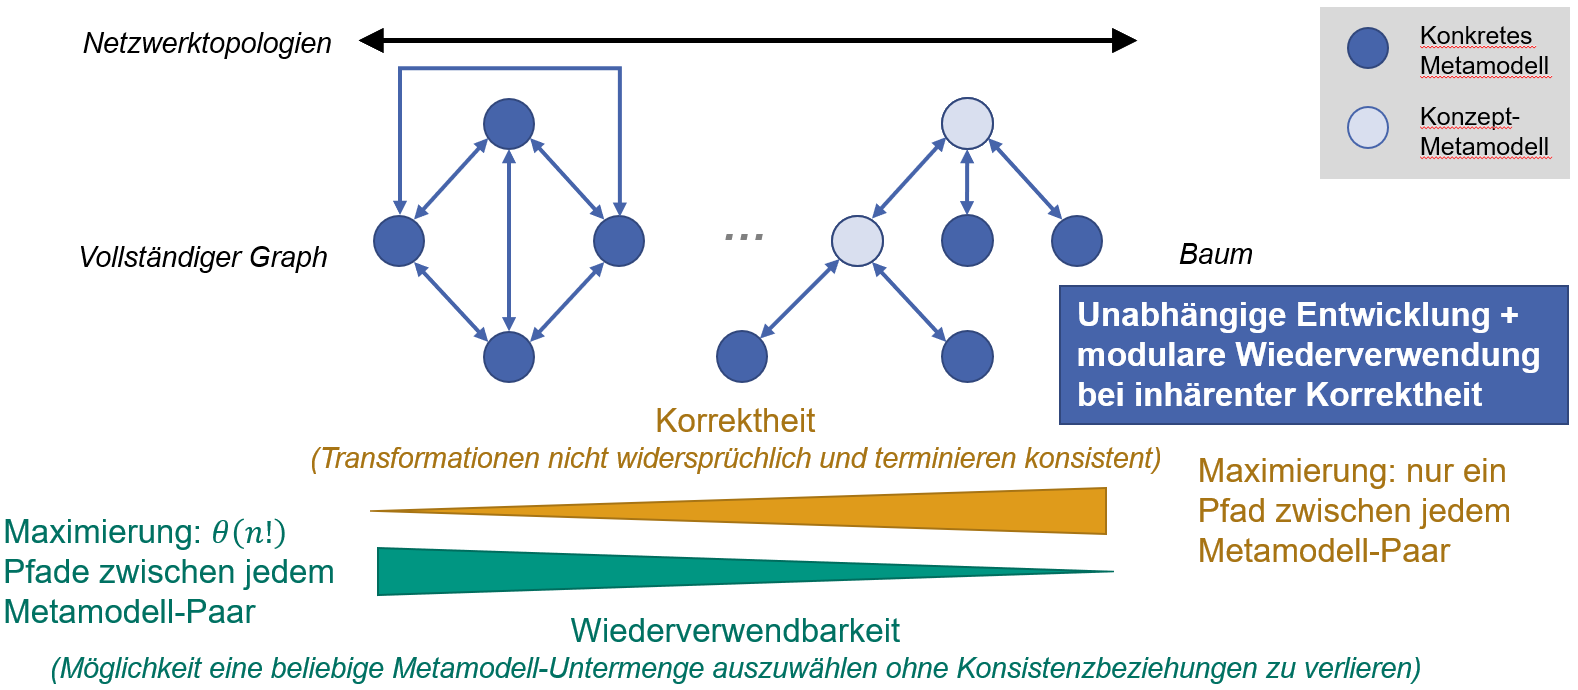
\includegraphics[width=\textwidth]{figures/quality/improvement/benefit_tradeoff.png}
%     \caption[Benefit of \commonalities regarding quality trade-offs]{Reduction of trade-off between quality properties using the \commonalities approach by ensuring correctness through a tree topology and achieving reusability by \concretemetamodels only being leaves.}
%     \label{fig:improvement:benefit_tradeoff}
% \end{figure}

% \todo{Instead of only discussion compatibility (which for sure is also true), discuss that in Commonalities there is always a consistent orchestration and that the shortest orchestration has an upper bound depending on the number of transformations. Discuss why this is not a drawback regarding such a bound in ordinary networks (especially discuss the previous example, where ping-pong was required, whereas here the required information is automatically added within the Commonalities and then only needs to be propagated back). However, there can still be scenarios that cannot be handled (due to the same reasons as for ordinary networks), but we already questioned there, although theoretically possible, whether they are practically relevant. In contrast to ordinary networks, Commonalities encode the limitation into the approach strategy and thus make it explicit for the developer rather then defining individual transformation without knowing how often they are executed later on. 
% -- Since the problem still remains, we did only discuss its mitigation already before}


\subsection{Reducing Specification Effort}

\mnote{Redundancies in consistency relations}
While the mitigation of the trade-off between correctness and reusability of a transformation network through the use of the \commonalities approach represents its major benefit, it can also reduce specification effort.
This is achieved by the fact each consistency relation must, in the best case, only be defined once, whereas in a transformation network inducing a dense or even complete graph, there need to be redundant representations of the same relations, at least if arbitrary parts of the network are supposed to be reusable.

\begin{figure}
    \centering
    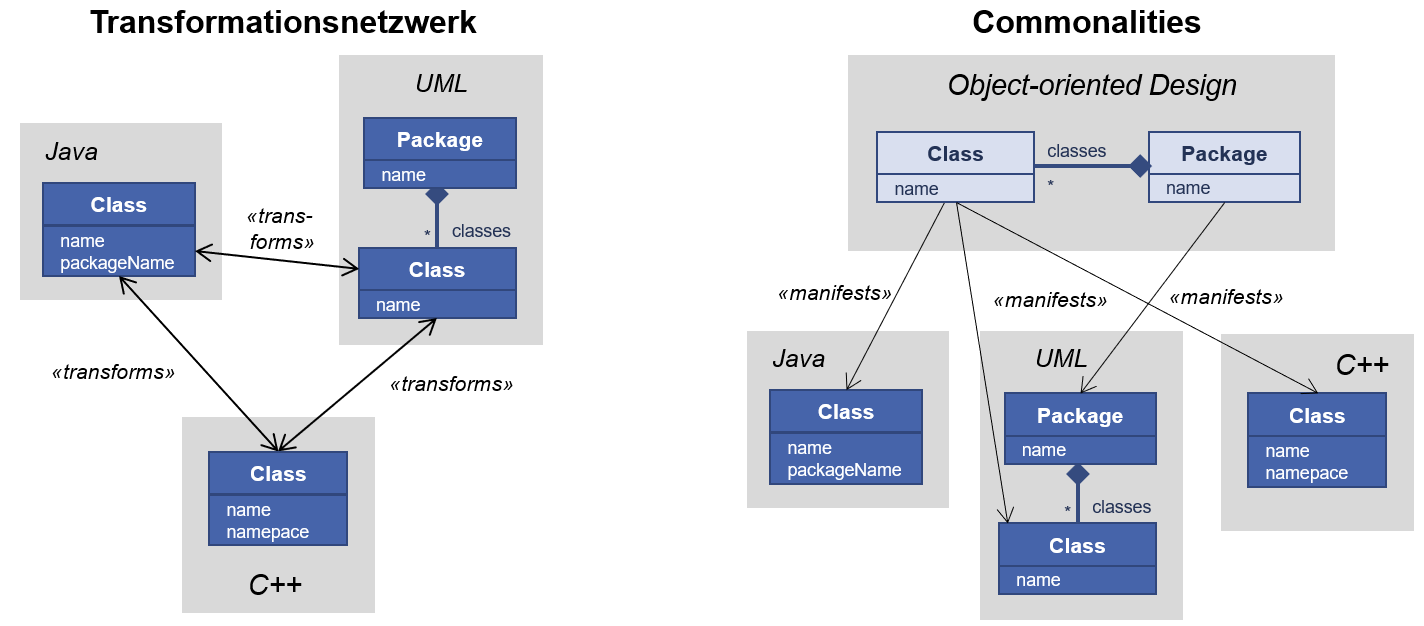
\includegraphics[width=\textwidth]{figures/quality/improvement/benefit_specification_effort.png}
    \caption[Benefit of \commonalities regarding specification effort]{Example for the number of defined relations with ordinary transformation networks and the usage of \conceptmetamodels with the \commonalities approach affecting the specification effort.}
    \label{fig:improvement:benefit_specification_effort}
\end{figure}

\mnote{Specification example}
\autoref{fig:improvement:benefit_specification_effort} depicts an the extension of introductory example given in \autoref{fig:improvement:running_example}, in which in addition to classes in \gls{UML} and Java a representation in \cplusplus is added.
In case of a transformation network, the relation between \cplusplus and both Java and \gls{UML} needs to be defined.
Using the \commonalities approach, only an additional manifestation relation to the concepts already defined in the object-oriented design \conceptmetamodels has to be specified.
In general, if $n$ metamodels share common concepts, adding an $n-1$-th metamodel requires $n$ transformations to be defined in ordinary networks, whereas the \commonalities approach, in the best case, only requires one addition manifestation relation to be defined.

\mnote{The average case}
The best case is, however, only achieved if the \conceptmetamodel already contains all information shared between the \concretemetamodel to be added and the ones for which the manifestation of the \commonalities in the \conceptmetamodel is already defined.
This is due to the already discussed fact that, informally speaking, the \conceptmetamodel needs to represent the union of all pairwise intersections of the \concretemetamodels.
Thus, usually it will be necessary to also extend or adapt the \conceptmetamodel and define or modify manifestations in the other \concretemetamodels as well.

\mnote{Initial effort}
In addition, applying the \commonalities approach may produce higher initial effort for the first consistency relations.
For two metamodels to keep consistent, one \conceptmetamodel and two manifestation relations, i.e., transformations, have to be defined instead of only a single transformation in case of directly relating the two metamodels.
This initial effort amortizes only if enough further \concretemetamodels are kept consistent via the same \conceptmetamodel.

\mnote{Initial effort reduction}
The initial specification effort can, however, also be reduced by providing a specific language to define \commonalities, which combines the definition of manifestation relations with the definition of its \commonality, such that the specification becomes nearly as concise as it would be if defined as a direct consistency relation between two metamodels.
We proposed such a language in \autoref{chap:language}.


% \begin{copiedFrom}{DocSym}

% This approach addresses all identified challenges % identified in \autoref{sec:approach:challenges} 
% and solves them under the assumption that all consistency relations %of a system 
% are described using \glspl{CMM}. %if their specification is encapsulated in a specialized language, our challenges identified in \autoref{sec:approach:challenges} can be addressed.
% %Under the assumption that all consistency relations of a system can be described using \acp{CMM}, we would be able to solve all identified challenges, as using \acp{CMM} allows to have the expressiveness of a graph of transformations, but abstracted to a tree structure with all its advantages.
% %We achieve \emph{uniqueness} by extracting common concepts into \acp{CMM} having to define only one relation of a metamodel to the \ac{CMM}. 
% We achieve inherent transformation compatibility by avoiding more than one transformation path %for the propagation of one change 
% between two metamodels by design. %Therefore, it is necessary to define \acp{CMM} relations in a way such that they induce a tree by also extracting common concepts of \acp{CMM} in other \acp{CMM}.  
% Since metamodels are only coupled across \glspl{CMM} and thus represent leaves of the transformation tree, any subset of them can be selected, maximizing modularity. % can be performed in a concrete usage scenario, maximizing modularity.
% %Finally, we assume that expressing consistency with explicit common concepts improves comprehensibility, %over combining binary consistency specifications
% %as it is a more natural representation and especially no transformations paths have to be traversed to understand a specific relation. % and expressing common information in common concepts is more natural than expressing it in transformations.
% %An approach of adding additional metamodels is also shortly discussed in \cite{stevens2020BidirectionalTransformationLarge-SoSym}, but with the focus on definability of multiary relations rather than the optimization regarding certain challenges.
% Finally, we assume that making common concepts explicit improves comprehensibility.

% \end{copiedFrom} % DocSym

% \begin{copiedFrom}{VoSE}

% % BENEFITS
% We expect several benefits from our approach, i.e. specifying \commonalities, in comparison to direct transformation specifications between metamodels.
% First, we claim to achieve \emph{better understandability} of relations between metamodels, because common concepts are made explicit. % rather than encoding them implicitly in transformations.
% Second, the approach \emph{reduces errors} when more than two metamodels are to be kept consistent.
% Transformations usually relate two metamodels, especially because multidirectional relations are hard to express~\cite{stevens2020BidirectionalTransformationLarge-SoSym},
% %\modified{either because the developer does not know about multidirectional relations or due to cognitive limitations~\cite{stevens2020BidirectionalTransformationLarge-SoSym},} %keep instances of two metamodels consistent 
% and therefore have to be combined to a network of transformations to keep instances of more than two metamodels consistent.
% % Following sentence moved from approach section
% Such a network can be regarded as a graph, formed by metamodels as its nodes and transformations as its edges.
% However, such a network can easily raise compatibility problems if there exists more than one path of transformations between two metamodels.
% A hierarchy of \commonality specifications is, by design, not prone to such problems.
% Finally, we \emph{improve reusability} in comparison to a network of transformations, %regarding a network of transformations, 
% because an arbitrary subset of metamodels, between which \commonalities are defined, can be selected to keep their instances consistent.
% In contrast, removing metamodels from a transformation network can easily lead to missing transformation paths between two metamodels.

% Benefits:
% \begin{itemize}
%     \item \emph{Better understandability} of relations, as common concepts are explicitly defined rather than implicitly encoding them in transformations
%     \item \emph{Improved reusability / partial usability} (regarding networks of binary transformations), because an arbitrary selection of concrete metamodels can be used and kept consistent
%     \item \emph{High expressiveness}, because no restriction due to predefined sets of statements, as expression can be added dynamically. This can be also improve analyzability of transformations, as additional metadata could be defined for each of the extensions.
% \end{itemize}

% \subsection*{Benefits of \commonalities}
% \label{chap:commonalities:approach:benefits}

% We suppose the \commonalities approach to provide two kinds of benefits:
% First, we expect that it improves understandability of relations between metamodels, because common concepts are not encoded in transformations implicitly but modelled explicitly.
% This is even a benefit if instances of only two metamodels shall be kept consistent.
% Second, it reduces problems that can occur if several bidirectional transformations are combined into a network of transformations to keep multiple models consistent.

% Two types of benefits:
% \begin{itemize}
%     \item Independent from network size: Understandability (explicit commonalities rather than implicit encoding in constraints)
%     \item Benefits for transformation networks (in the following)
% \end{itemize}

% \begin{figure}
%     \centering
%     \begin{minipage}[b]{0.49\columnwidth}
%         \centering
%         \newcommand{\hmmdistance}{3.6em}
\newcommand{\vmmdistance}{2.4em}

\begin{tikzpicture}[
    mm/.style={schematic metamodel},
]

\node[mm] (full_left) {};
\node[mm, above right=\vmmdistance and \hmmdistance of full_left.center, anchor=center] (full_top) {};
\node[mm, below right=\vmmdistance and \hmmdistance of full_left.center, anchor=center] (full_bottom) {};
\node[mm, right=2*\hmmdistance of full_left.center, anchor=center] (full_right) {};
\node[mm, below left=\vmmdistance and \hmmdistance of full_left.center, anchor=center] (full_bottomleft) {};

\draw[transformation] (full_left) -- (full_top);
\draw[transformation] (full_left) -- (full_right);
\draw[transformation] (full_left) -- (full_bottom);
\draw[transformation] (full_top) -- (full_right);
\draw[transformation] (full_top) -- (full_bottom);
\draw[transformation] (full_right) -- (full_bottom);
\draw[transformation] (full_left) -- (full_bottomleft);
\draw[transformation] (full_bottom) -- (full_bottomleft);
\draw[transformation] (full_top) to[bend right=30] (full_bottomleft);
\draw[transformation] (full_bottomleft) .. controls ++(1*\hmmdistance, -0.8*\vmmdistance) and ([yshift=-1.5*\vmmdistance]full_right.south) .. (full_right);

\end{tikzpicture}
%         \subcaption{Dense Graph}
%         \label{fig:improvement:topologies:full}
%     \end{minipage}
%     \hfill
%     \begin{minipage}[b]{0.49\columnwidth}
%         \centering
%         \newcommand{\hmmdistance}{3.6em}
\newcommand{\vmmdistance}{2.4em}

\begin{tikzpicture}[
    conceptmm/.style={schematic conceptmetamodel},
    concretemm/.style={schematic metamodel},
]

\node[conceptmm, right=4*\hmmdistance of full_left.center, anchor=center] (tree_left) {};
\node[conceptmm, above right=\vmmdistance and \hmmdistance of tree_left.center, anchor=center] (tree_top) {};
\node[concretemm, below right=\vmmdistance and \hmmdistance of tree_left.center, anchor=center] (tree_bottom) {};
\node[concretemm, right=2*\hmmdistance of tree_left.center, anchor=center] (tree_right) {};
\node[concretemm, below left=\vmmdistance and \hmmdistance of tree_left.center, anchor=center] (tree_bottomleft) {};

\draw[transformation] (tree_left) -- (tree_top);
\draw[transformation] (tree_left) -- (tree_bottom);
\draw[transformation] (tree_left) -- (tree_bottomleft);
\draw[transformation] (tree_top) -- (tree_right);

\end{tikzpicture}
%         \vspace{1em}
%         \subcaption{Tree}
%         \label{fig:improvement:topologies:tree}
%     \end{minipage}
%     \caption[Extremes of transformation network topologies]{Extremes of transformation network topologies: nodes represent metamodels, edges represent transformations (\conceptmetamodels in a tree of \commonalities in dark gray). Adapted from~\owncite[Fig. 4]{klare2019models}.}
%     \label{fig:improvement:topologies}
% \end{figure}

% Networks of transformations can have two extremes of topologies, as depicted in \autoref{fig:improvement:topologies}.
% If transformations between all metamodels are defined, the network forms a dense graph (see \autoref{fig:improvement:topologies:full}).
% In contrast, if there exists exactly one path of transformations between each pair of metamodels, the network forms a tree (see \autoref{fig:improvement:topologies:tree}).
% Several properties for such %transformation 
% networks have been identified by \textcite{gleitze2017a} and \textcite{klare2018docsym}.
% Two essential properties %, defined in \cite{klare2018docsym}, 
% are \emph{compatibility} and \emph{modularity}~\cite{klare2018docsym}, which, unfortunately, contradict each other.
% The \commonalities approach, however, improves both of them. %, which is an essential benefit that we discuss in the following. %We discuss the benefits of the \commonalities approach regarding those properties.
% \emph{Compatibility} means that transformations do not define contradictory constraints.
% Consider the relations introduced for the running example in \autoref{fig:improvement:running_example}.
% The names of the same class in Java and UML are defined to be equal.
% If a class in Java and UML realizes a \gls{PCM} component, it shall have the same name appended with an \enquote{Impl} suffix.
% If transformations realize the three relations between \gls{PCM}, UML and Java, and the one between \gls{PCM} and Java adds that suffix whereas the one between \gls{PCM} and UML omits it, the constraints can never be fulfilled.
% %If the three relations between Java, UML and \ac{PCM} are defined in transformations and the one between \ac{PCM} and Java adds that suffix whereas the one between \ac{PCM} and UML omits it, the constraints can never be fulfilled.
% In that case, the transformations are considered incompatible.
% Incompatibility may arise whenever more than one transformation path between two metamodels exists.
% In consequence, compatibility cannot be guaranteed in dense network, whereas it is inherently high if the network forms a tree.
% \emph{Modularity} means that any subset of the metamodels can be used without loosing consistency because of missing transformations.
% Modularity is high if any metamodel can be removed from the network and the remaining transformations still define consistency between all remaining metamodels.
% In consequence, modularity is high in a dense network, because all metamodels are directly related, while it is low if the network is a tree, because inner nodes cannot be removed without their children not being related by a transformation anymore.
% Since redundant paths between metamodels improve modularity but reduce compatibility, these properties are inherently contradicting.

% The \commonalities approach improves both these properties due to the fact that additional metamodels are introduced in the specification.
% The transformations between \metaclasses in \concretemetamodels and \commonalities in \conceptmetamodels induce a tree, thus compatibility is high.
% Additionally, only the leaves of the tree are \concretemetamodels, which are actually used to describe a system and whose instances are modified, whereas the inner nodes only represent auxiliary metamodels, exemplarily marked in \autoref{fig:improvement:topologies:tree}. 
% In consequence, taking an arbitrary subset of \concretemetamodels removes only leaves and can thus be done without removing any transformations that are necessary to keep instances of the remaining metamodels consistent.
% This constitutes a major benefit of the \commonalities approach as compared to ordinary networks of transformations.


% \subsection{Limitations of \commonalities}
% \label{sec:approach:limitations}
% ONE PART MOVED TO COMPOSITION (DAG INSTEAD OF TREES), ONE MOVED TO LIMITATIONS IN EVALUATION SECTION

% \end{copiedFrom} % VoSE


\section{Application Processes}
\label{chap:improvement:application}

\mnote{Definition process}
The application of the \commonalities approach requires a process for defining them as well a concept for combining them with other specifications of transformations.
In a specification using the \commonalities approach, the \conceptmetamodels and manifestation relations are not as independent as they are supposed to be in the definition of an ordinary transformation network forming a dense or even complete graph.
Due to the necessity to relate all elements only via one transformation path, even if \commonalities are separated into \conceptmetamodels by concerns and composed hierarchically, the developers must ensure that such a structure is achieved.
We thus subsequently discuss different options how \commonalities can be defined.

\mnote{Combination concept}
We have identified in \autoref{chap:improvement:concepts:specification} that the \commonalities approach is well-suited for structural and \enquote{natural} consistency relations, rather than arbitrarily complex, in particular behavioral dependencies.
%This especially involves structural rather than behavioral consistency relations.
In the following, we discuss options for combining a \commonalities specification with other specifications, in particular ordinary transformations.


\subsection{Defining \Commonalities}

\mnote{Hierarchic composition}
We have discussed in \autoref{chap:improvement:commonalities:composition} how \commonalities and the \conceptmetamodels encapsulating them can be composed hierarchically.
This allows to separate \commonalities by concerns, i.e., by the concepts they belong to.
In addition, it fosters the independent development and reuse of different \conceptmetamodels.

\mnote{Independent development vs. tree structure}
The \commonalities approach does, however, only provide an essential benefit regarding guaranteed correctness of the resulting transformation network if the manifestation relations specify consistency relations that form a consistency relation tree (see \autoref{chap:improvement:commonalities:tree}).
Thus, \commonalities and their \conceptmetamodels must be composed in a way that such a structure is achieved.
This can, in the worst case, require all \concretemetamodels to define consistency between and the according relations to be elicited a priori and thus conflict with our independent development assumption.

\mnote{Bottom-up specification}
An intuitive process to define \commonalities is a bottom-up approach.
Developers select \concretemetamodels that share common concepts and are, by custom definition, most related among the \concretemetamodels to define consistency between and define a \conceptmetamodel of \commonalities between them.
Then, they iteratively choose \conceptmetamodels, and potentially also \concretemetamodels, that share further higher-level commonalities and define an according \conceptmetamodel for them.
This ends up in a hierarchy of \conceptmetamodels.

\mnote{Driven by \concretemetamodels}
Since finally instances of the \concretemetamodels are to be kept consistent, it is important to always consider the information represented in the \concretemetamodels, even if consistency is defined between \conceptmetamodels, i.e., at a higher level in the hierarchy of \conceptmetamodels.
Consider the running example of classes in \gls{UML} and Java, as well as components in \gls{UML}.
We may define an object-oriented design \conceptmetamodel to define \commonalities between \gls{UML} and Java, as well as a component-based design \conceptmetamodel to define \commonalities between object-oriented design and \gls{PCM}, as sketched in \autoref{chap:improvement:commonalities:tree} and depicted in \autoref{fig:improvement:composed_commonalities_example}.
If these \conceptmetamodels are defined in a bottom-up manner, i.e., first defining the object-oriented design \conceptmetamodel and afterwards the component-based design \conceptmetamodels, it is not sufficient to only consider the information represented in the object-oriented design \conceptmetamodels for defining their \commonalities.
That metamodel does only contain the \commonalities that are relevant for object-oriented design, but for the relation to component-based design, further information that is only present in one of the \concretemetamodels may be relevant.
For example, Java contains a definition of behavior in terms of method bodies, which is not represented in the purely structural \gls{UML} class models.
Thus, the object-oriented design \conceptmetamodel does not represent this behavioral information, as it does represent a \commonality.
\gls{PCM}, however, also has an abstract representation of behavior used for predicting the system's performance, which needs to be kept consistent with the precise behavior specification in Java.
Thus, the component-based design \conceptmetamodel must either have an additional manifestation relation to Java for the behavioral information, or the object-oriented design \conceptmetamodel must also contain behavioral information, although not being a \commonality between the \concretemetamodels it represents.

\mnote{Union of all information}
In general, this problem occurs because \conceptmetamodels are supposed to represent the unions of all pairwise intersections of their \concretemetamodels, as those represent the \commonalities that have to be kept consistent.
Information that is unique to one of the \concretemetamodels is not represented in the \conceptmetamodel, but may be relevant for further concepts and thus the relations to define to them.
A first, general solution would require a \conceptmetamodel to contain the union of all information in the \concretemetamodels rather than the union of their pairwise intersections.
This does, however, not conform to the purpose of \conceptmetamodels to only describe \commonalities.
It leads to large and complex \conceptmetamodels and thus also to high effort, because for each \concretemetamodel a transformation, in terms of a manifestation relation, of all its information to a \conceptmetamodel would have to be defined.
In addition, the topmost \conceptmetamodel of the hierarchy would inherently contain the union of information defined in all \concretemetamodels, thus representing a \gls{SUMM}, i.e., a single metamodel that is capable of representing all information to define one system (see \autoref{chap:foundations:multiview}). %, as introduced in \autoref{chap:improvement:concepts:explicit}.
In consequence, it would be sufficient to only manage an instance of that topmost \conceptmetamodel, representing the \gls{SUMM}, and to consider the instances of all other concept and \concretemetamodels as projections from the instance of that central metamodel, according to \textcite{atkinson2010a}.

\begin{figure}
    \centering
    \newcommand{\vdistance}{8em}
\newcommand{\hdistance}{14em}
\newcommand{\classwidth}{5.5em}
\newcommand{\labeldistance}{1em}
\newcommand{\labelshift}{0.3*\classwidth}
\newcommand{\mmborder}{1em}

\begin{tikzpicture}

\pgfdeclarelayer{bg}
\pgfsetlayers{bg,main}


% METACLASSES

\umlclassvarwidth{java_class}{}{Class}{
name\\
visbility\\
** behavior **
}{\classwidth}

\umlclassvarwidth[, right=0.8*\hdistance of java_class.north, anchor=north]{uml_class}{}{Class}{
name\\
visbility\\
}{\classwidth} 

\umlclassvarwidth[, above right=1.1*\vdistance and 0.5*\hdistance of java_class.north, anchor=north]{oo_class}{}{Class\vphantom{p}}{
name\\
visibility\\
** behavior **
}{\classwidth} 

\umlclassvarwidth[, right=\hdistance of oo_class.north, anchor=north]{pcm_component}{}{Component}{
name\\
** behavior **
}{\classwidth} 

\umlclassvarwidth[, above right=1.1*\vdistance and 0.5*\hdistance of oo_class.north, anchor=north]{component_component}{}{Component}{
name\\
visbility\\
** behavior **
}{\classwidth}

% METAMODELS

\coordinate (java_label_coordinate) at ([yshift=\labeldistance]java_class.north west);
\node[mmlabel, anchor=west] (java_label) at (java_label_coordinate) {Java};

\coordinate (uml_label_coordinate) at ([yshift=\labeldistance]uml_class.north east);
\node[mmlabel, anchor=east] (uml_label) at (uml_label_coordinate) {\acrshort{UML}};

\coordinate (oo_label_coordinate) at ([xshift=-4*\labelshift,yshift=\labeldistance]oo_class.north);
\node[mmlabel, anchor=west, align=left] (oo_label) at ([xshift=-0.5em, yshift=-0.7em]oo_label_coordinate) {Object-oriented\\ Design};

\coordinate (pcm_label_coordinate) at ([yshift=\labeldistance]pcm_component.north east);
\node[mmlabel, anchor=east] (pcm_label) at (pcm_label_coordinate) {\acrshort{PCM}};

\coordinate (component_label_coordinate) at ([yshift=\labeldistance]component_component.north);
\node[mmlabel, anchor=center] (component_label) at (component_label_coordinate) {Component-based Design};

\begin{pgfonlayer}{bg}
    \node[mmbg, fit=(java_class)(java_label.west), inner sep=\mmborder] (java) {};
    \node[mmbg, fit=(uml_class)(uml_label.east), inner sep=\mmborder] (uml) {};
    \node[conceptmmbg, fit=(oo_class)(oo_label_coordinate), inner sep=\mmborder] (oo) {};
    \node[mmbg, fit=(pcm_component)(pcm_label.east), inner sep=\mmborder] (pcm) {};
    \node[conceptmmbg, fit=(component_component)(component_label.west)(component_label.east), inner sep=\mmborder] (component) {};
\end{pgfonlayer}


% CONSISTENCY RELATIONS

\draw[manifests relation] (oo_class) -- node[manifests relation, above, sloped] {\manifestslabel} (java_class);
\draw[manifests relation] (oo_class) -- node[manifests relation, above, sloped] {\manifestslabel} (uml_class);
\draw[manifests relation] (component_component) -- node[manifests relation, above, sloped] {\manifestslabel} (oo_class);
\draw[manifests relation] (component_component) -- node[manifests relation, above, sloped] {\manifestslabel} (pcm_component);

\end{tikzpicture}

    \caption[\Commonalities with union of all information]{Example for a hierarchy of \conceptmetamodels and their \commonalities, in which \conceptmetamodels represent the union of information in their manifestations. Behavior of classes and components is considered any, not further specified kind of behavioral information.}
    \label{fig:improvement:definition_option_sum}
\end{figure}

\mnote{Example for union}
For the example int \autoref{fig:improvement:composed_commonalities_example} depicting hierarchic \conceptmetamodels for classes and components, we derive an extension according to the discussed scheme in \autoref{fig:improvement:definition_option_sum}.
It additionally contains visibilities for classes and any kind of not further specified behavior description in Java classes and \gls{PCM} components.
Both \conceptmetamodels contain the union information in their manifestations, such that the component-based design \conceptmetamodel contains all information represented in all metamodels.
In consequence, the component-based design \conceptmetamodel represents the visibility of classes in object-oriented design, although it is not relevant for components and is not kept consistent via that \conceptmetamodel.

\mnote{Non-strict manifestations}
The previous considerations assume a kind of strict layered architecture (see~\cite{buschmann1996PatternsArchitecture-Book}) in which the manifestation relations induce a tree between the metamodels, thus no manifestation relation bypasses a \conceptmetamodel to whose \commonalities additional manifestation relations are defined.
Referring to a non-strict layered architecture, another solution would be to allow manifestation relations to the manifestations of \conceptmetamodels to which further manifestation relations are defined, e.g., the component-based design \commonalities may have manifestation relations to elements in Java and \gls{UML} in addition to manifestation relations to the object-oriented design \conceptmetamodels, which in turn has manifestation relations to those \concretemetamodels.
A drawback of this solution is that it can likely violate the goal of achieving a tree structure.
Considering a class in Java as a manifestation of a component in component-based design, as well as a class in object-oriented design, which in turn is a manifestation of a component in component-based design, would already violate the definition of a consistency relation tree, thus not giving guarantees regarding compatibility.

\begin{figure}
    \centering
    \newcommand{\vdistance}{8em}
\newcommand{\hdistance}{14em}
\newcommand{\classwidth}{5.5em}
\newcommand{\labeldistance}{1em}
\newcommand{\labelshift}{0.3*\classwidth}
\newcommand{\mmborder}{1em}

\begin{tikzpicture}

\pgfdeclarelayer{bg}
\pgfsetlayers{bg,main}


% METACLASSES

\umlclassvarwidth{java_class}{}{Class}{
name\\
visbility\\
** behavior **
}{\classwidth}

\umlclassvarwidth[, right=0.8*\hdistance of java_class.north, anchor=north]{uml_class}{}{Class}{
name\\
visbility\\
}{\classwidth} 

\umlclassvarwidth[, above right=\vdistance and 0.5*\hdistance of java_class.north, anchor=north]{oo_class}{}{Class\vphantom{p}}{
name\\
visibility\\
}{\classwidth} 

\umlclassvarwidth[, right=\hdistance of oo_class.north, anchor=north]{pcm_component}{}{Component}{
name\\
** behavior **
}{\classwidth} 

\umlclassvarwidth[, above right=\vdistance and 0.5*\hdistance of oo_class.north, anchor=north]{component_component}{}{Component}{
name\\
** behavior **
}{\classwidth}

% METAMODELS

\coordinate (java_label_coordinate) at ([yshift=\labeldistance]java_class.north west);
\node[mmlabel, anchor=west] (java_label) at (java_label_coordinate) {Java};

\coordinate (uml_label_coordinate) at ([yshift=\labeldistance]uml_class.north east);
\node[mmlabel, anchor=east] (uml_label) at (uml_label_coordinate) {\acrshort{UML}};

\coordinate (oo_label_coordinate) at ([xshift=-4*\labelshift,yshift=\labeldistance]oo_class.north);
\node[mmlabel, anchor=west, align=left] (oo_label) at ([xshift=-0.5em, yshift=-0.7em]oo_label_coordinate) {Object-oriented\\ Design};

\coordinate (pcm_label_coordinate) at ([yshift=\labeldistance]pcm_component.north east);
\node[mmlabel, anchor=east] (pcm_label) at (pcm_label_coordinate) {\acrshort{PCM}};

\coordinate (component_label_coordinate) at ([yshift=\labeldistance]component_component.north);
\node[mmlabel, anchor=center] (component_label) at (component_label_coordinate) {Component-based Design};

\begin{pgfonlayer}{bg}
    \node[mmbg, fit=(java_class)(java_label.west), inner sep=\mmborder] (java) {};
    \node[mmbg, fit=(uml_class)(uml_label.east), inner sep=\mmborder] (uml) {};
    \node[conceptmmbg, fit=(oo_class)(oo_label_coordinate), inner sep=\mmborder] (oo) {};
    \node[mmbg, fit=(pcm_component)(pcm_label.east), inner sep=\mmborder] (pcm) {};
    \node[conceptmmbg, fit=(component_component)(component_label.west)(component_label.east), inner sep=\mmborder] (component) {};
\end{pgfonlayer}


% CONSISTENCY RELATIONS

\draw[manifests relation] (oo_class) -- node[stereotype, above, sloped] {\manifestslabel} (java_class);
\draw[manifests relation] (oo_class) -- node[stereotype, above, sloped] {\manifestslabel} (uml_class);
\draw[manifests relation] (component_component) -- node[stereotype, above, sloped] {\manifestslabel} (oo_class);
\draw[manifests relation] (component_component) -- node[stereotype, above, sloped] {\manifestslabel} (pcm_component);
\draw[manifests relation] (component_component) .. controls ([yshift=-0.5em,xshift=-\hdistance]component_component.west) and ([yshift=2*\vdistance]java_class.north west) .. ([xshift=-0.5em]java_class.north) node[stereotype, pos=0.25, above] {\manifestslabel};

\end{tikzpicture}

    \caption[\Commonalities with multiple manifestations]{Example for a hierarchy of \conceptmetamodels and their \commonalities, in which \commonalities may have several manifestations inducing consistency relations that do not form a tree structure. Behavior of classes and components is considered any, not further specified kind of behavioral information.}
    \label{fig:improvement:definition_option_bypass}
\end{figure}

\mnote{Example for non-strict manifestations}
\autoref{fig:improvement:definition_option_bypass} depicts this solution for the already discussed example.
The \conceptmetamodels contain only the information relevant for the \commonalities they represent.
The additional manifestation relation between components of the component-based design \conceptmetamodel and classes in Java induce the violation of a tree structure as sketched before.
Although behavior may actually be represented in terms of method bodies represented as separate \metaclasses in Java, still consistency relations defined by the manifestation relations between Java and the object-oriented design \conceptmetamodel would include both classes and methods, as methods do not share an isolated consistency relation between Java and \gls{UML} but only in the context of the class they belong to.

\mnote{Union including concepts}
A third option is to construct a \conceptmetamodel not only driven by the \commonalities shared between its manifestations, but also by its \commonalities with other metamodels.
Thus, whenever a \conceptmetamodel is used as a manifestation of another \conceptmetamodel, it may be extended by the information from its manifestations required for the \commonalities in another concept with other metamodels.
For example, as soon as the object-oriented design \conceptmetamodel is considered as a manifestation of component-based design, its manifestations, namely Java and \gls{UML}, are checked for \commonalities with component-based design that are not yet considered \commonalities regarding object-oriented design.
This could be a description of method bodies in Java to keep consistent with the behavior specification in \gls{PCM}.
If consequently followed, such an approach would result in \conceptmetamodels not only representing the union of the pairwise intersections of the manifestations, but the union of the pairwise intersections of their manifestations with all other \concretemetamodels to be kept consistent.
This still promises to lead to \conceptmetamodels that are significantly smaller and more precise than the union of all metamodels as in the first option, but still allow to achieve a tree structure, which is why we propose to use this option.
This approach is comparable to the situation in which a further manifestation shall be added, like we exemplarily discussed for adding \cplusplus as a manifestation of the object-oriented design \conceptmetamodel in \autoref{chap:improvement:benefits:specification_effort}.

\begin{figure}
    \centering
    \newcommand{\vdistance}{7.7em}
\newcommand{\hdistance}{14em}
\newcommand{\classwidth}{5.5em}
\newcommand{\labeldistance}{1em}
\newcommand{\labelshift}{0.3*\classwidth}
\newcommand{\mmborder}{1em}

\begin{tikzpicture}

\pgfdeclarelayer{bg}
\pgfsetlayers{bg,main}


% METACLASSES

\umlclassvarwidth{java_class}{}{Class}{
name\\
visbility\\
** behavior **
}{\classwidth}

\umlclassvarwidth[, right=0.8*\hdistance of java_class.north, anchor=north]{uml_class}{}{Class}{
name\\
visbility\\
}{\classwidth} 

\umlclassvarwidth[, above right=1.2*\vdistance and 0.5*\hdistance of java_class.north, anchor=north]{oo_class}{}{Class\vphantom{p}}{
name\\
visibility\\
** behavior **
}{\classwidth} 

\umlclassvarwidth[, right=\hdistance of oo_class.north, anchor=north]{pcm_component}{}{Component}{
name\\
** behavior **
}{\classwidth} 

\umlclassvarwidth[, above right=\vdistance and 0.5*\hdistance of oo_class.north, anchor=north]{component_component}{}{Component}{
name\\
** behavior **
}{\classwidth}

% METAMODELS

\coordinate (java_label_coordinate) at ([yshift=\labeldistance]java_class.north west);
\node[mmlabel, anchor=west] (java_label) at (java_label_coordinate) {Java};

\coordinate (uml_label_coordinate) at ([yshift=\labeldistance]uml_class.north east);
\node[mmlabel, anchor=east] (uml_label) at (uml_label_coordinate) {UML};

\coordinate (oo_label_coordinate) at ([xshift=-4*\labelshift,yshift=\labeldistance]oo_class.north);
\node[mmlabel, anchor=west, align=left] (oo_label) at ([xshift=-0.5em, yshift=-0.7em]oo_label_coordinate) {Object-oriented\\ Design};

\coordinate (pcm_label_coordinate) at ([yshift=\labeldistance]pcm_component.north east);
\node[mmlabel, anchor=east] (pcm_label) at (pcm_label_coordinate) {PCM};

\coordinate (component_label_coordinate) at ([yshift=\labeldistance]component_component.north);
\node[mmlabel, anchor=center] (component_label) at (component_label_coordinate) {Component-based Design};

\begin{pgfonlayer}{bg}
    \node[mmbg, fit=(java_class)(java_label.west), inner sep=\mmborder] (java) {};
    \node[mmbg, fit=(uml_class)(uml_label.east), inner sep=\mmborder] (uml) {};
    \node[conceptmmbg, fit=(oo_class)(oo_label_coordinate), inner sep=\mmborder] (oo) {};
    \node[mmbg, fit=(pcm_component)(pcm_label.east), inner sep=\mmborder] (pcm) {};
    \node[conceptmmbg, fit=(component_component)(component_label.west)(component_label.east), inner sep=\mmborder] (component) {};
\end{pgfonlayer}


% CONSISTENCY RELATIONS

\draw[manifests relation] (oo_class) -- node[manifests relation, above, sloped] {\manifestslabel} (java_class);
\draw[manifests relation] (oo_class) -- node[manifests relation, above, sloped] {\manifestslabel} (uml_class);
\draw[manifests relation] (component_component) -- node[manifests relation, above, sloped] {\manifestslabel} (oo_class);
\draw[manifests relation] (component_component) -- node[manifests relation, above, sloped] {\manifestslabel} (pcm_component);

\end{tikzpicture}

    \caption[\Commonalities including information of their concepts]{Example for a hierarchy of \conceptmetamodels and their \commonalities, in which \commonalities represent information necessary for the concepts they are manifestations of in addition to the information shared by their manifestations. Behavior of classes and components is considered any, not further specified kind of behavioral information.}
    \label{fig:improvement:definition_option_super_union}
\end{figure}

\mnote{Example for union including concepts}
The application of this option to the already discussed example is depicted in \autoref{fig:improvement:definition_option_super_union}.
In this solution, still a tree structure between the \metaclasses and \commonalities is given and the \conceptmetamodels are still restricted to the information in the manifestations and, in addition, the information of the manifestations necessary for the \conceptmetamodels of which they are manifestations.
This is why the object-oriented design \conceptmetamodel contains information about the behavior of classes and components, although \gls{UML} and Java do not share behavioral concepts, but the component \commonality for component-based design does not contain the visibilities of classes as in the first option of representing the union of all information in the manifestations.

\mnote{Problem mitigation by cliques}
Finally, it is still an open question how problematic the actual dependencies in practical scenarios are.
Potentially, only subsets of few metamodels are highly related and share large parts of one or more concepts, and the relation to other such subsets is only given across one metamodel or one concept.
This could be seen as a graph of cliques, in which some metamodels are highly related whereas the relation to others is rather loose.
In that case, it can be reasonable to define relations in these cliques by means of \commonalities and then define the loose relations to other cliques by means of an ordinary transformation, as we discuss in the subsequent section.
We derive first insights on the achievability of the required tree structure for \commonalities in our evaluation in \autoref{chap:commonalities_evaluation}, but further evidence if one of the previously discussed strategies can be reasonably applied has to be gained in larger studies in practical scenarios with more metamodels of more tools.

% Discuss how commonalities can be defined. Which roles are involved, especially how different domain experts can communicate. E.g., bottom-up approach: Take the most related metamodels and define their commonalities. Then define higher-level commonalities relating these concept metamodels or even the concrete metamodels. 
% The problem is that combining two concept metamodels requires them to contain all necessary information, thus a concept metamodel design is not only driven by the metamodels to keep directly consistent, but also by the information that is needed to preserve consistency to other commonalities. This refers to the same scenario as if multiple commonality structures are encapsulated into projective view environments which are combined by BX. They require the exposed views to provide all information necessary to preserve consistency.

% Prozess zur Erzeugung von Commonalities beschreiben:
% - Optimalerweise kennt man alle MM vorher und kann sinnvolle Commonalities bauen (immer das am wenigstens redundante Konstrukt, z.B. eher Person in Familie als Persons mit Familiennamen (redundante Darstellung des Familiennamens)
% - Bei Erweiterung um zusätzliche Metamodelle sind ggf. Anpassungen an Commonalities notwendig. Hier ist wieder die Lokalität bei den Commonalities vorteilhaft (interne Spezifikation), weil man dann eine Commonality insgesamt ersetzen kann statt in jeder Transformation deren Manifestierung anzupassen.

% Evolutionsprozess:
% - Wie eignet sich welcher Ansatz zur Erweiterung mit MM. I.d.R. reicht es nicht eine Verbindung zu ergänzen, sondern die Konzeptmetamodelle für angepasst werden für ein neuen zu koppelndes Metamodell


\subsection{Combining \Commonalities}

\mnote{Necessity for combination}
We have up to now discussed how to construct \conceptmetamodels and manifestation relations in terms of the \commonalities approach, such that the topology of the defined relations fulfills the definition of a consistency relation tree to achieve inherent guarantees regarding correctness of the transformation network.
We have also derived how the \commonalities approach improves reusability in comparison to the construction of a transformation network with tree topology out of the \concretemetamodels.
Nevertheless, the approach has at least two limitations, which we have already identified.
First, it lacks completeness, as it requires a specific topology of consistency relations to be achievable, which is likely to get more complex the more metamodels are involved.
Second, it only fits well for structural relations in which actual commonalities can be described or prescribed.

\mnote{\Commonalities for subsets}
In consequence, to improve applicability of the approach, it should be applied for subsets of metamodels that inherently share commonalities, comparable to the cliques mentioned before, which are suited to be described with the proposed approach.
These specifications should then be combined with other consistency specifications, be they defined with the \commonalities approach or with ordinary transformations.
Such a combination would restrict the size and complexity of a hierarchy of \commonalities and could foster reuse of consistency specifications for specific concepts in different context, as motivated by our assumptions of independent development and modular reuse, as well as the process proposed in \autoref{chap:networks:specification_process}.

\begin{figure}
    \centering
    \newcommand{\mmdistance}{8em}

\begin{tikzpicture}[
    mm/.style={schematic metamodel},
    conceptmm/.style={schematic conceptmetamodel}
]

\node[mm] (original_left) {$\metamodel{A}{}$};
\node[mm, right=\mmdistance of original_left.center, anchor=center] (original_middle) {$\metamodel{B}{}$};
\node[mm, right=\mmdistance of original_middle.center, anchor=center] (original_right) {$\metamodel{C}{}$};
\node[conceptmm, above right=0.8*\mmdistance and 0.5*\mmdistance of original_left.center, anchor=center, align=center] (concept) {$\metamodel{AB}{\mathvariable{Concepts}}$};

\draw[consistency relation] (original_left) -- node[above] {$\consistencyrelation{CR}{AB}$} (original_middle);
\draw[consistency relation] (original_middle) to[bend left=30] node[above] {$\consistencyrelation{CR}{BC}$} (original_right);
\draw[consistency relation] (original_left) to[bend right=35] node[above] {$\consistencyrelation{CR}{AC}$} (original_right);

\draw[consistency relation, color=gray] (original_left) -- node[above left=-0.3em and 0.5em] {$\consistencyrelation{CR}{A}$} (concept);
\draw[consistency relation, color=gray] (original_middle) -- node[above right=-0.3em and 0.3em] {$\consistencyrelation{CR}{B}$} (concept);
\draw[consistency relation, color=gray] (original_right) to[bend right=30] node[pos=0.6, below left] {$\consistencyrelation{CR}{C}$} (concept);


\node[right=3*\mmdistance+0.4*\difftoafiveimage of concept.north, anchor=north east, align=left] (constraints_top) { 
$\consistencyrelation{CR}{AB} \concat \consistencyrelation{CR}{BC} \neq (\consistencyrelation{CR}{AB} \concat \consistencyrelation{CR}{BC}) \cap \consistencyrelation{CR}{AC} \neq \consistencyrelation{CR}{AC}$
};

\node[below=2em of constraints_top.north east, anchor=north east, align=left] {
$\consistencyrelation{CR}{A} \concat \consistencyrelation{CR}{B} = \consistencyrelation{CR}{AB}$\\
$\consistencyrelation{CR}{A} \concat \consistencyrelation{CR}{C} = \consistencyrelation{CR}{AC}$\\
$\consistencyrelation{CR}{B} \concat \consistencyrelation{CR}{C} = \consistencyrelation{CR}{BC}$\\
};

\end{tikzpicture}
    \caption[Partial transformation network of \commonalities]{Example for a \conceptmetamodel $\metamodel{AB}{\mathvariable{Concepts}}$ to replace a consistency relation, and the replacement of ordinary consistency relations to the \concretemetamodels with one to the \conceptmetamodel. Adapted from~\owncite[Fig.~5]{klare2018docsym}.}
    \label{fig:improvement:commonalities_combination_generic}
\end{figure}

\mnote{General combination requirements}
To preserve the benefits of a \commonalities specification, it can be combined with other specifications, be they ordinary transformations or another \commonalities specification, by considering any of the other metamodels as a manifestation or a \conceptmetamodel of one of the \conceptmetamodels of the \commonalities specifications.
This preserves the tree structures of the \commonalities specification and its benefits.
Consider the generic example in \autoref{fig:improvement:commonalities_combination_generic} with three metamodels, a \conceptmetamodel for two of them and consistency relations between them, which are considered \modellevelconsistencyrelations according to \autoref{def:modellevelconsistencyrelation} for reasons of simplicity.
The consistency relation $\consistencyrelation{CR}{AB}$ between metamodels $\metamodel{A}{}$ and $\metamodel{B}{}$ is expressed by a \conceptmetamodel $\metamodel{AB}{\mathvariable{Concepts}}$ and consistency relations for the according manifestation relations $\consistencyrelation{CR}{A}$ and $\consistencyrelation{CR}{B}$.
In addition, the metamodel $\metamodel{C}{}$ shares consistency relations with both other metamodels.
To preserve reusability and the necessary tree structure, these consistency relations $\consistencyrelation{CR}{AB}$ and $\consistencyrelation{CR}{AC}$ should be described in terms of a consistency relation $\consistencyrelation{CR}{C}$ to the concept metamodel.
This does, however, require the \conceptmetamodel to contain all information that is necessary to preserve consistency between $\metamodel{C}{}$ and the two others, as described with the required relations in \autoref{fig:improvement:commonalities_combination_generic}.
In contrast to the scenarios discussed in the previous section for how to define \conceptmetamodels and which information to put into them, if $\metamodel{C}{}$ is a part of a different consistency specification to combine the \commonalities specification with, or if the \commonalities specification covers more than two \concretemetamodels with one \conceptmetamodel, this can require an arbitrarily complex adaptation, which may even not be wanted of possible at all if modular reuse is desired.

\mnote{Virtualization by views}
To improve such a combination of specifications, virtualization concepts as known from \gls{OSM}~\cite{atkinson2010a} (see \autoref{chap:foundations:multiview:osm}) and the \vitruv approach~\owncite{klare2021Vitruv-JSS} (see \autoref{chap:foundations:multiview:vitruv}) can be applied.
Their idea is to encapsulate metamodels and their instances behind a facet of views and to enable access to the actual models only via these views.
Views are projections of the encapsulated models, i.e., they derive all information from the models and potentially aggregate them or arrange them differently.
The metamodels of these views are called \emph{\viewtypes}.
While those approaches were originally designed to provide a well-defined interface through views for developers and internally ensure consistency of the persisted artifacts by either avoiding or managing redundancy, they can also be used as an interface for consistency preservation.
In the \vitruv approach, a so called \gls{VSUM} is composed of models and rules for preserving their consistency, whose contents are exposed by views to be modified by developers.

\begin{figure}
    \centering
    % requires tikzvitruvius.sty
\begin{tikzpicture}[
    vtcaption/.style={font=\small},
    view/.style={uml box, densely dashed},
    viewtype/.style={circle, draw, solid, fill=white, inner sep=.1em, font=\scriptsize},
    polarrow/.style={latex-latex, densely dotted},
    mininode/.style={inner sep=.4em},
    uniformly sized package/.style={minimum width=2.5em},
]

% V-SUM
\umlpackage[uniformly sized package]{oo}{}{OOD}
\umlpackage[uniformly sized package]{uml}{below left=4.5em and 0em of oo}{\acrshort{UML}}
\umlpackage[uniformly sized package]{java}{below right=4.5em and 0em of oo}{Java}

\node[circle,draw,thick,fit=(oo.center)(uml)(java),inner sep=2ex] (sum) {};

\draw[manifests relation] (oo) -- node[manifests relation, above, sloped] (pcmJavaCCR) {\manifestslabel} (uml.north);
\draw[manifests relation] (oo) -- node[manifests relation, above, sloped] (pcmJavaCCR) {\manifestslabel} (java.north);

\node[viewtype] (viewtypeOO) at (sum.60) {$\mathvariable{VT}_\mathvariable{OOD}$};
\node[viewtype] (viewtypeJava) at (sum.5) {$\mathvariable{VT}_\mathvariable{Java}$};
\draw[polarrow] (oo) -- (viewtypeOO);
\draw[polarrow] (java) -- (viewtypeJava);

\node[font=\bfseries\footnotesize] (sumtext) [above=0.6em of sum.270, anchor=south, align=center] {\vsum\\ Metamodel};

% Outer transformations
\umlpackage[uniformly sized package]{pcm}{above right=-0.5em and 13em of oo}{\acrshort{PCM}};
\draw[transformation] (viewtypeOO) -- node[transformation, above, sloped] {Structure} (pcm);
\draw[transformation] (viewtypeJava) -- node[transformation, above, sloped] {Behavior} (pcm);

% Legend
\node[draw, legendbg, matrix, font=\scriptsize, inner sep=0.7em, nodes=mininode] (legend) at (17.5em,-5.8em) {%
    \umlpackage[minimum height=0.1em, inner sep=0.3em, yshift=0.5ex, font=\scriptsize, xshift=1.25em]{legend_mm}{}{MM} & \node[anchor=base west, font=\footnotesize] {Metamodel\sameheight};\\
    \node[viewtype, xshift=1.25em, yshift=0.5ex, font=\scriptsize] {$\mathvariable{VT}$}; & \node[anchor=base west, font=\footnotesize] {\ViewType\sameheight};\\
    \draw[polarrow] (0,.5ex)--(2.5em,.5ex); & \node[anchor=base west, font=\footnotesize] {View Transformation\sameheight};\\
    \draw[transformation] (0,.5ex)--(2.5em,.5ex); & \node[anchor=base west, font=\footnotesize] {Transformation\sameheight};\\
};

\end{tikzpicture}

    %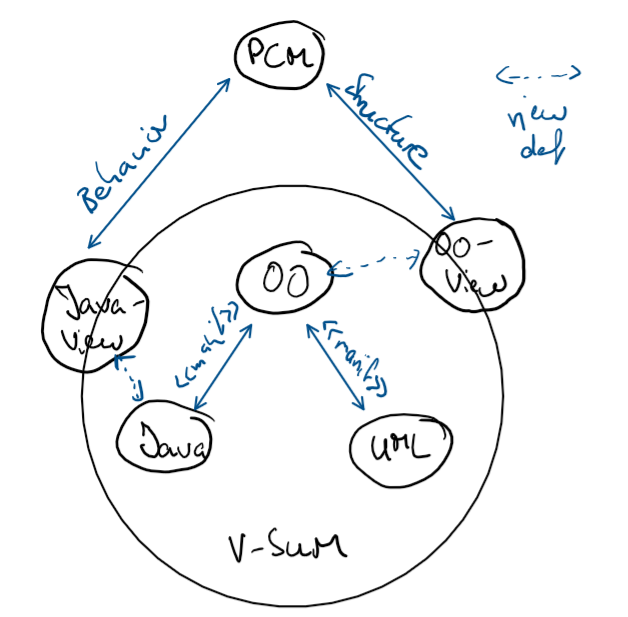
\includegraphics[width=0.6\textwidth]{figures/quality/improvement/combination_external_metamodel.png}
    \caption[Combination of \commonalities with a transformation]{Example for the combination of a \commonalities specification for object-oriented design (OOD) with \gls{PCM} by encapsulation into a \vsumm.}
    \label{fig:improvement:combination_external_metamodel}
\end{figure}

\mnote{Encapsulation of \commonalities in \vsum}
Consider the example depicted in \autoref{fig:improvement:combination_external_metamodel}.
It comprises the \commonalities specification for Java and \gls{UML} using a single \conceptmetamodel for object-oriented design.
This consistency specification by means of \commonalities is encapsulated into a \vsum, which exposes the Java code via a Java view and the object-oriented structure represented in instances of the \conceptmetamodel as an object-oriented view.
These two views are then related to \gls{PCM} by means of ordinary consistency relations and transformations preserving them.
The relations between metamodels and \viewtypes can, again, be considered ordinary transformations.
Thus, the defined transformation network would actually contain cycles, such that it does not benefit from the \commonalities specification within the \vsum in terms of correctness.
If we do only consider the \vsum itself, it does, however, still have a tree structure, so if only one of the views is modified at the same time, it provides the benefits that we have discussed for a \commonalities specification in \autoref{chap:improvement:benefits}.
In addition, views of a \vsum by now actually assume that only one of them is changed at a time~\owncite{klare2021Vitruv-JSS}, as a developer is supposed to work on one specific view at a time.
Thus, if the transformations outside the \vsum ensure that only one of the views is changed at a time, the \vsum provides the discussed benefits of the \commonalities approach.

\mnote{Clarification of responsibilities}
This approach does, of course, not solve possible issues regarding synchronization and orchestration in the transformation network defined outside the \vsum, but only moves the problem of avoiding these issues away from the \commonalities specification by making according assumptions in terms of allowing only modifications of one view of a \vsum.
It does, however, clarify responsibilities, as there are precisely defined views across which other metamodels can be combined with those for which consistency is defined by means of \commonalities, rather than defining consistency to the metamodels within the \commonalities specification directly and thus breaking the necessary assumption for the intended benefits of that approach.
In the example, we have a clear separation into views for the structure of the object-oriented representation in Java, \gls{UML} and potentially more metamodels, and for its behavior.
It is up to the developer of the transformation network outside the \vsum to ensure that no problems like execution loops occur by assigning clear non-conflicting responsibilities to the two transformations for structure and behavior of the \vsum to \gls{PCM}.

\begin{figure}
    \centering
    % requires tikzvitruvius.sty
\begin{tikzpicture}[
    vtcaption/.style={font=\small},
    view/.style={uml box, densely dashed},
    viewtype/.style={circle, draw, solid, fill=white, inner sep=.1em, font=\scriptsize},
    polarrow/.style={latex-latex, densely dotted},
    mininode/.style={inner sep=.4em},
    uniformly sized package/.style={minimum width=2.5em},
]

% V-SUM 1
\umlpackage[uniformly sized package]{oo}{}{OOD}
\umlpackage[uniformly sized package]{uml}{below left=4.5em and 0em of oo}{UML}
\umlpackage[uniformly sized package]{java}{below right=4.5em and 0em of oo}{Java}

\node[circle,draw,thick,fit=(oo.center)(uml)(java),inner sep=2ex] (sum1) {};

\draw[manifests relation] (oo) -- node[manifests relation, above, sloped] (pcmJavaCCR) {\manifestslabel} (uml.north);
\draw[manifests relation] (oo) -- node[manifests relation, above, sloped] (pcmJavaCCR) {\manifestslabel} (java.north);

\node[viewtype] (viewtypeOO) at (sum1.40) {$\mathvariable{VT}_\mathvariable{OOD}$};
\node[viewtype] (viewtypeJava) at (sum1.5) {$\mathvariable{VT}_\mathvariable{Java}$};
\draw[polarrow] (oo) -- (viewtypeOO);
\draw[polarrow] (java) -- (viewtypeJava);

\node[font=\bfseries\footnotesize] (sum1text) [above=0.6em of sum1.270, anchor=south, align=center] {\vsum\\ Metamodel};

% V-SUM 2
\umlpackage[uniformly sized package]{cbd}{right=14.8em of oo}{CBD}
\umlpackage[uniformly sized package]{pcm}{below left=4.5em and 0em of cbd}{PCM}
\umlpackage[uniformly sized package]{umlcomp}{below right=4.5em and 0em of cbd}{UML}

\node[circle,draw,thick,fit=(cbd.center)(pcm)(umlcomp),inner sep=2ex] (sum2) {};

\draw[manifests relation] (cbd) -- node[manifests relation, above, sloped] (pcmJavaCCR) {\manifestslabel} (pcm.north);
\draw[manifests relation] (cbd) -- node[manifests relation, above, sloped] (pcmJavaCCR) {\manifestslabel} (umlcomp.north);

\node[viewtype] (viewtypeStruc) at (sum2.140) {$\mathvariable{VT}_\mathvariable{Structure}$};
\node[viewtype] (viewtypeBehav) at (sum2.175) {$\mathvariable{VT}_\mathvariable{Behavior}$};
\draw[polarrow] (cbd) -- (viewtypeStruc);
\draw[polarrow] (pcm.north west) -- (viewtypeBehav);

\node[font=\bfseries\footnotesize] (sum2text) [above=0.6em of sum2.270, anchor=south, align=center] {\vsum\\ Metamodel};

% Outer transformations
\draw[transformation] (viewtypeOO) -- (viewtypeStruc);
\draw[transformation] (viewtypeJava) -- (viewtypeBehav);

\coordinate (middle) at ($(oo)!0.5!(cbd)$);

% Legend
\node[draw, legendbg, matrix, font=\scriptsize, inner sep=0.7em, nodes=mininode, anchor=north, below=10.5em of middle] (legend) {%
    \umlpackage[minimum height=0.1em, inner sep=0.3em, yshift=0.5ex, font=\scriptsize, anchor=center]{legend_mm}{}{MM} & \node[anchor=base west, font=\footnotesize] {Metamodel \hspace{0.5em}\sameheight}; &
    \draw[polarrow] (0em,0.5ex)--(2em,0.5ex); & \node[anchor=base west, font=\footnotesize] {View Transformation\sameheight}; \\
    \node[viewtype, anchor=center, yshift=0.5ex, font=\scriptsize] {$\mathvariable{VT}$}; & \node[anchor=base west, font=\footnotesize] {\ViewType\sameheight};&
    \draw[transformation] (0em,0.5ex)--(2em,0.5ex); & \node[anchor=base west, font=\footnotesize] {Transformation\sameheight};\\
};

\end{tikzpicture}

    %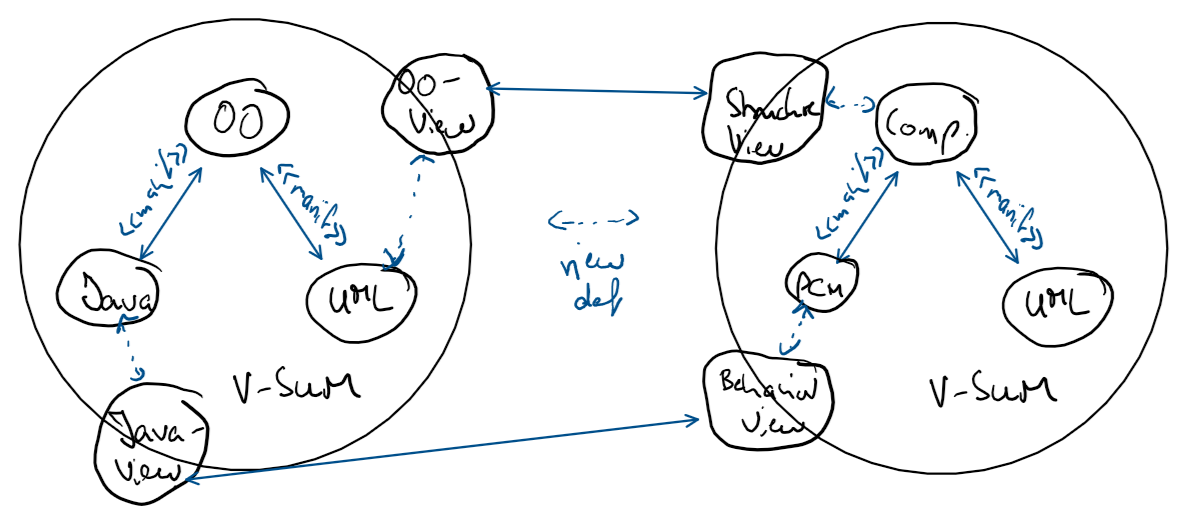
\includegraphics[width=\textwidth]{figures/quality/improvement/combination_two_vsums.png}
    \caption[Combination of two \commonalities specifications]{Example for the combination of two \commonalities specifications for object-oriented (OOD) and component-based design (CBD) by encapsulation into \vsumms.}
    \label{fig:improvement:combination_two_vsums}
\end{figure}

\mnote{Combination of encapsulating \vsums}
Instead of only \gls{PCM}, there could be a more complex transformation network, or another \commonalities specification, which may again be encapsulated into a \vsum and provide its own views, across which both \vsums can then be combined.
\autoref{fig:improvement:combination_two_vsums} depicts such an example, in which \gls{PCM} and \gls{UML} component models are related by a \conceptmetamodel for component-based design, encapsulated into a second \vsum.
This \vsum provides separate \viewtypes for the structure represented by both \gls{PCM} and \gls{UML} and thus reflected in the \conceptmetamodels, and for the behavior only represented in \gls{PCM}.
These \viewtypes can then be combined by means of ordinary transformations with those of the \vsum for object-oriented design.
Again, this approach does not prevent the occurrence of correctness issues as discussed in \autoref{part:correctness} due to the transformations outside the \vsum, but at least within each \vsum we can guarantee correctness.

\mnote{Hierachic composition of \vsums}
This approach can even be hierarchically be composed, such that several kinds of specifications, including encapsulating \vsums, are again encapsulated into another \vsum.
For example, the \vsums in \autoref{fig:improvement:combination_two_vsums} could be encapsulated into a \vsum for object-oriented and component-based design to be reused together.
If the transformation network between the inner \vsums is correct, which can also be achieved by defining \commonalities between the views of these \vsums again, the composed \vsum again guarantees correctness and can provide well-defined views for different concerns of component-based and object-oriented design.

\mnote{Required evidence}
The sketched approaches for combining \commonalities specification with other kinds of consistency specifications have to be considered as conceptual ideas which promise to provide the benefits of specifying modular, reusable specifications that ease the achievement of correctness.
They have, however, not been applied yet. 
Thus, their actual applicability still has to be practically evaluated in case studies.


\section{Summary}

In this section, we have discussed how the insights regarding effects of different network topologies on the quality properties of a transformation network can be used to mitigate trade-offs between them.
We have motivated a different way of considering consistency in terms of making common concepts explicit as \emph{commonalities} instead of implicitly encoding them into consistency relations.
We have used this way of specifying consistency to propose a construction approach for transformation networks that results in a tree topology providing inherent benefits regarding correctness, but also provides high reusability due to the actual metamodels, whose instances are used to describe a system, being leaves of the tree induces by the transformation network.
We conclude this chapter with the following central insight.

\begin{insight}[Trade-off Mitigation]
    Quality properties of transformation networks are influenced by the network's topology.
    Especially correctness and reusability are contrary properties, which induce a trade-off depending on whether the network topology is rather a dense or a sparse graph.
    The drawback regarding reusability in networks with tree topology arises from the fact that the metamodels represented by the inner nodes of the tree cannot be easily omitted, as consistency between several other metamodels is expressed across them.
    This can be mitigated by ensuring that the metamodels represented by the inner nodes are auxiliary artifacts and not the actual metamodels used by developers.
    This matches with a different way of thinking about consistency in terms of making the commonalities between metamodels to keep consistent explicit in addition metamodels rather than encoding them implicitly in consistency relations.
    Following such a specification approach leads to a network that improves both correctness and reusability, which are contradictory if only considering transformations between the metamodels whose instances are actually used by developers.
    Such an approach can even be used to define consistency partially for some of the metamodels and then combine it with other consistency specifications, such as ordinary transformations.
    To still have the same guarantees regarding correctness and reusability, such a specification can be encapsulated behind views, which provide projections of the information within the actual models and do only allow one of them to be updated at a time.
\end{insight}
